\documentclass[11pt]{article}
\usepackage[T1]{fontenc}
\usepackage[utf8]{inputenc}
\usepackage[margin=1in]{geometry}
\usepackage{amsmath,amssymb,amsthm}
\usepackage{tikz}
\usepackage{float}
\usepackage{comment}
% Use \showproofstrue to show proofs; \showproofsfalse to hide them.
\newif\ifshowproofs
\showproofsfalse
\ifshowproofs
\else
  % Keep each \begin{proof} and \end{proof} on its own line.
  \excludecomment{proof}
\fi
\usepackage{microtype}
\usepackage[hidelinks]{hyperref}
\newcommand{\E}{\mathbb E}
\newcommand{\Pb}{\mathbb P}
\newcommand{\Ind}[1]{\mathbf 1\{#1\}}
\newtheorem{proposition}{Proposition}
\newtheorem{lemma}{Lemma}
\newtheorem{corollary}{Corollary}
\newtheorem{theorem}{Theorem}
\title{Final note: Intermediate forgetting}
\author{Standalone theoretical note}
\date{}
\begin{document}
\maketitle

Here we gather the results of intermediate forgetting rates. First we provide an equivalent condition based on the fixed policy of using always product 1 where the maximum advantage is positive and hence, product 2 is used. This result allows us to characterize the conditions under which product 2 is used, using a policy that is easier to implement. 


\begin{proposition}[Characterization of positive advantage]
\label{prop:positive-characterization}
Let $U^{1}_\rho$ be the value of always choosing product~1.
For $\rho\in(0,1)$, we have $\mathcal A_\rho>0$ if and only if
\begin{equation}
\max_{z\in\mathcal K_\rho}
\left[U_\rho^1(T_\rho^s z)-U_\rho^1(T_\rho^f z)\right]
>\frac{\Delta c}{\gamma\Delta p}.
\end{equation}
\end{proposition}

\begin{proof}
Conditional on a purchase from seller~$A$, let
\begin{equation*}
Q_\rho^i(z)
=R-c_i+\gamma\left[p_iU_\rho^1(T_\rho^s z)
+(1-p_i)U_\rho^1(T_\rho^f z)\right],
\qquad i\in\{1,2\}.
\end{equation*}
This is the value of choosing product~$i$ for the current purchase and
product~1 thereafter. Subtracting the two expressions gives
\begin{equation*}
Q_\rho^2(z)-Q_\rho^1(z)
=-\Delta c+\gamma\Delta p
\left[U_\rho^1(T_\rho^s z)-U_\rho^1(T_\rho^f z)\right].
\end{equation*}
Define
\begin{equation*}
\mathcal A_\rho^1
=\max_{z\in\mathcal K_\rho}
\left\{-\Delta c+\gamma\Delta p
\left[U_\rho^1(T_\rho^s z)-U_\rho^1(T_\rho^f z)\right]\right\}.
\end{equation*}
The fixed-policy operator is a contraction preserving continuity,
so $U_\rho^1$ is continuous and this maximum exists.
We first show that $\mathcal A_\rho>0$ if and only if
$\mathcal A_\rho^1>0$, by proving that their nonpositivity conditions
are equivalent.

Suppose $\mathcal A_\rho^1\leq0$. Then
$ Q_\rho^1(z)\geq Q_\rho^2(z)$ at every
$z\in\mathcal K_\rho$. By the fixed-policy Bellman equation,
\begin{equation*}
U_\rho^1(z)
=\frac{D_\rho(z)}{1-\gamma[1-D_\rho(z)]}Q_\rho^1(z)
=\frac{D_\rho(z)}{1-\gamma[1-D_\rho(z)]}
\max_{i\in\{1,2\}} Q_\rho^i(z).
\end{equation*}
Thus $U_\rho^1$ also satisfies the optimal Bellman equation on
$\mathcal K_\rho$. Since this set is invariant under both transitions,
the Bellman operator restricted to it is a contraction. Uniqueness
therefore gives $U_\rho^1=V_\rho$ on $\mathcal K_\rho$, and hence
$\mathcal A_\rho=\mathcal A_\rho^1\leq0$.

Conversely, suppose $\mathcal A_\rho\leq0$. Product~1 then maximizes
the Bellman expression evaluated at $V_\rho$ at every state in
$\mathcal K_\rho$. Consequently, $V_\rho$ satisfies the Bellman equation
for always choosing product~1 on this invariant set. Uniqueness of
the fixed-policy value gives $V_\rho=U_\rho^1$ there, and hence
$\mathcal A_\rho^1=\mathcal A_\rho\leq0$.

We have proved $\mathcal A_\rho\leq0$ if and only if
$\mathcal A_\rho^1\leq0$. Taking negations gives the desired equivalence
of strict positivity. Finally, since $\Delta c$ and $\gamma\Delta p>0$
do not depend on $z$,
\begin{equation*}
\mathcal A_\rho^1
=-\Delta c+\gamma\Delta p\max_{z\in\mathcal K_\rho}
\left[U_\rho^1(T_\rho^s z)-U_\rho^1(T_\rho^f z)\right].
\end{equation*}
Therefore $\mathcal A_\rho^1>0$ is equivalent to the inequality
in the statement.
\end{proof}

Second, we prove that, when the maximum advantage is positive, product 2 is used not only once but infinitely often. This result is for every $\rho \in (0,1)$ where $\mathcal A_\rho>0$. 


\begin{proposition}[Persistent use of product~2]
\label{prop:persistence}
If $\mathcal A_\rho>0$, then there is a constant
$\eta>0$, such that
\begin{equation}
\liminf_{N\to\infty}\frac1N\sum_{n=1}^{N}\Ind{i_n=2}\geq\eta
\qquad\text{a.s},
\end{equation}
where $i_n$ is the product chosen at the $n$th interaction with the provider~$A$.
In particular, product~2 is used infinitely often.
\end{proposition}

\begin{proof}
Fix an optimal policy and an initial state $x_0\in\mathcal Z$.
Throughout the proof, $x=(x_s,x_f)$ denotes the full normalized
state in
\begin{equation*}
\mathcal Z=\{(x_s,x_f):x_s\ge0,\ x_f\ge0,\ x_s+x_f\le1\},
\end{equation*}
and $\|\cdot\|$ denotes the Euclidean norm.
Let $x_n$ be the state after the $n$th interaction with provider A.
Thus, product $i_n$ is chosen at state $x_{n-1}$.

Since $D_\rho$ is continuous and strictly positive on the compact
set $\mathcal Z$, it is bounded below by a positive constant.
Consequently, each successive interaction with provider A occurs
in finite calendar time almost surely, so the interaction sequence
is well defined.

To locate states where product 2 is uniquely optimal, define,
for every $x\in\mathcal Z$,
\begin{equation*}
a_\rho(x)
:=-\Delta c+\gamma\Delta p
\left[
V_\rho(T_\rho^s(x))-V_\rho(T_\rho^f(x))
\right].
\end{equation*}
By continuity of $V_\rho$ and the transition maps,
$a_\rho$ is continuous on $\mathcal Z$.
Since $\mathcal K_\rho$ is compact, the maximum
\begin{equation*}
\mathcal A_\rho
=\max_{x\in\mathcal K_\rho}a_\rho(x)
\end{equation*}
is attained. Choose $x^*\in\mathcal K_\rho$ such that
\begin{equation*}
a_\rho(x^*)=\mathcal A_\rho>0.
\end{equation*}

By continuity at $x^*$, there exists $\varepsilon>0$ such that,
for all $x\in\mathcal Z$,
\begin{equation*}
\|x-x^*\|<\varepsilon
\quad\Longrightarrow\quad
|a_\rho(x)-\mathcal A_\rho|
<\frac{\mathcal A_\rho}{2}.
\end{equation*}
In particular,
\begin{equation}
\label{eq:pers-neighborhood}
\|x-x^*\|<\varepsilon
\quad\Longrightarrow\quad
a_\rho(x)>
\mathcal A_\rho-\frac{\mathcal A_\rho}{2}
=\frac{\mathcal A_\rho}{2}>0.
\end{equation}

Here $a_\rho(x)$ is the difference between the values of choosing
products 2 and 1, conditional on a purchase from provider A and
with optimal continuation in both cases.
Therefore, product 2 is uniquely optimal at every state in this
neighborhood.

We next show that a single finite outcome sequence brings every
starting state into this neighborhood. For any
$x,\widetilde x\in\mathcal Z$, applying the success transition
to both states gives
\begin{equation*}
\begin{aligned}
T_\rho^s(x)-T_\rho^s(\widetilde x)
&=(\rho x_s+1-\rho,\rho x_f)
 -(\rho\widetilde x_s+1-\rho,\rho\widetilde x_f)\\
&=\rho(x_s-\widetilde x_s,x_f-\widetilde x_f)\\
&=\rho(x-\widetilde x).
\end{aligned}
\end{equation*}
The same identity holds for a failure.
Hence, for either $o\in\{s,f\}$,
\begin{equation*}
\|T_\rho^o(x)-T_\rho^o(\widetilde x)\|
=\rho\|x-\widetilde x\|.
\end{equation*}

For a sequence $w=(w_1,\ldots,w_m)\in\{s,f\}^m$,
listed in chronological order, write
\begin{equation*}
T_\rho^w
:=T_\rho^{w_m}\circ\cdots\circ T_\rho^{w_1}.
\end{equation*}
Repeated application of the preceding identity yields
\begin{equation}
\label{eq:pers-contraction}
\|T_\rho^w(x)-T_\rho^w(\widetilde x)\|
=\rho^m\|x-\widetilde x\|.
\end{equation}

Since the diameter of $\mathcal Z$ is $\sqrt{2}$,
choose an integer $m\ge1$ such that
\begin{equation*}
\sqrt{2}\,\rho^m<\varepsilon.
\end{equation*}
This choice of $m$ does not depend on the starting state.

The invariance identity
\begin{equation*}
\mathcal K_\rho
=T_\rho^s(\mathcal K_\rho)\cup T_\rho^f(\mathcal K_\rho),
\end{equation*}
iterated $m$ times, gives
\begin{equation*}
\mathcal K_\rho
=\bigcup_{w\in\{s,f\}^m}T_\rho^w(\mathcal K_\rho).
\end{equation*}
Because $x^*\in\mathcal K_\rho$, there exist a sequence
$w\in\{s,f\}^m$ and a state
$\widetilde x\in\mathcal K_\rho$ such that
\begin{equation*}
T_\rho^w(\widetilde x)=x^*.
\end{equation*}

Fix this sequence $w$.
For every starting state $x\in\mathcal Z$,
\begin{equation}
\label{eq:pers-word}
\begin{aligned}
\|T_\rho^w(x)-x^*\|
&=\|T_\rho^w(x)-T_\rho^w(\widetilde x)\|\\
&=\rho^m\|x-\widetilde x\|\\
&\le\sqrt{2}\,\rho^m<\varepsilon.
\end{aligned}
\end{equation}
Thus, the same sequence $w$ brings every starting state into
the neighborhood in \eqref{eq:pers-neighborhood}.

To bound the probability of this sequence conditional on past
observations, let $\mathcal F_n$ denote the complete history
through the outcome of interaction $n$, including the initial
state and past product choices.
Set
\begin{equation*}
q:=\min\{p_1,1-p_2\}>0.
\end{equation*}

At every interaction, regardless of the chosen product,
the conditional probability of success is at least $p_1$,
and that of failure is at least $1-p_2$.
Therefore,
\begin{equation*}
\begin{aligned}
\Pr(\text{success at interaction }n+1\mid\mathcal F_n)
&\ge p_1\ge q,\\
\Pr(\text{failure at interaction }n+1\mid\mathcal F_n)
&\ge1-p_2\ge q,
\end{aligned}
\qquad\text{almost surely}.
\end{equation*}

By successive conditioning, the conditional probability that
the next $m$ outcomes equal the fixed sequence $w$ is at least
$q^m$, regardless of the previous history.
This does not require independence between outcomes or blocks.

Divide the interactions into consecutive, nonoverlapping blocks
of length $m$.
Block $k$ contains interactions
\begin{equation*}
(k-1)m+1,\ldots,km.
\end{equation*}
Define the indicator
\begin{equation*}
X_k
:=\mathbf 1\{
\text{the outcomes in block }k\text{ equal }w
\}.
\end{equation*}
Then
\begin{equation}
\label{eq:pers-block-bound}
\mathbb E[X_k\mid\mathcal F_{(k-1)m}]
=\Pr(X_k=1\mid\mathcal F_{(k-1)m})
\ge q^m
\qquad\text{almost surely}.
\end{equation}

To turn \eqref{eq:pers-block-bound} into an almost-sure frequency
bound, define $M_0=0$ and, for $k\ge1$,
\begin{equation*}
M_k
:=\sum_{j=1}^{k}
\left(
X_j-\mathbb E[X_j\mid\mathcal F_{(j-1)m}]
\right).
\end{equation*}
We verify that $(M_k)_{k\ge0}$ is a martingale with respect to
$(\mathcal F_{km})_{k\ge0}$.

First, $X_j$ is $\mathcal F_{jm}$-measurable and
$\mathbb E[X_j\mid\mathcal F_{(j-1)m}]$ is
$\mathcal F_{(j-1)m}$-measurable.
For $j\le k$,
\begin{equation*}
\mathcal F_{(j-1)m}
\subseteq\mathcal F_{jm}
\subseteq\mathcal F_{km}.
\end{equation*}
Thus, every term in $M_k$ is determined by the history available
after block $k$, so $M_k$ is $\mathcal F_{km}$-measurable.

Second, since $X_j$ and its conditional expectation belong
to $[0,1]$,
\begin{equation*}
\left|
X_j-\mathbb E[X_j\mid\mathcal F_{(j-1)m}]
\right|\le1.
\end{equation*}
Consequently,
\begin{equation*}
\mathbb E[|M_k|]
\le
\mathbb E\!\left[
\sum_{j=1}^{k}
\left|
X_j-\mathbb E[X_j\mid\mathcal F_{(j-1)m}]
\right|
\right]
\le k<\infty.
\end{equation*}
In fact, $|M_k|\le k$, so
$\mathbb E[M_k^2]\le k^2<\infty$ as well.

Third, separating the last increment and taking conditional
expectations gives
\begin{equation*}
\begin{aligned}
\mathbb E[M_k\mid\mathcal F_{(k-1)m}]
&=M_{k-1}
+\mathbb E\!\left[
X_k-\mathbb E[X_k\mid\mathcal F_{(k-1)m}]
\mid\mathcal F_{(k-1)m}
\right]\\
&=M_{k-1}
+\mathbb E[X_k\mid\mathcal F_{(k-1)m}]
-\mathbb E[X_k\mid\mathcal F_{(k-1)m}]\\
&=M_{k-1}.
\end{aligned}
\end{equation*}
This establishes the martingale property.

Also, the tower property gives
\begin{equation*}
\mathbb E\!\left[
X_j-\mathbb E[X_j\mid\mathcal F_{(j-1)m}]
\right]
=\mathbb E[X_j]-\mathbb E[X_j]=0,
\end{equation*}
so $\mathbb E[M_k]=0$ for every $k$.

To obtain almost-sure convergence, observe that
\begin{equation*}
|M_k-M_{k-1}|
=
\left|
X_k-\mathbb E[X_k\mid\mathcal F_{(k-1)m}]
\right|
\le1.
\end{equation*}
Hence
\begin{equation*}
\mathbb E[(M_k-M_{k-1})^2]\le1,
\end{equation*}
and therefore
\begin{equation*}
\sum_{k=1}^{\infty}
\frac{\mathbb E[(M_k-M_{k-1})^2]}{k^2}
\le
\sum_{k=1}^{\infty}\frac{1}{k^2}
<\infty.
\end{equation*}
The martingale strong law, in the form of
\cite[Exercise~4.4.11]{Durrett2019} with $b_k=k$,
now yields
\begin{equation}
\label{eq:pers-martingale-limit}
\frac{M_k}{k}\longrightarrow0
\qquad\text{almost surely}.
\end{equation}

By the definition of $M_k$ and \eqref{eq:pers-block-bound},
\begin{equation*}
\begin{aligned}
\frac{1}{k}\sum_{j=1}^{k}X_j
&=
\frac{1}{k}\sum_{j=1}^{k}
\mathbb E[X_j\mid\mathcal F_{(j-1)m}]
+\frac{M_k}{k}\\
&\ge q^m+\frac{M_k}{k}.
\end{aligned}
\end{equation*}
Taking lower limits and using
\eqref{eq:pers-martingale-limit}, we obtain
\begin{equation}
\label{eq:pers-block-frequency}
\liminf_{k\to\infty}
\frac{1}{k}\sum_{j=1}^{k}X_j
\ge q^m
\qquad\text{almost surely}.
\end{equation}

It remains to relate these block occurrences to choices of product 2.
If $X_j=1$, then \eqref{eq:pers-word} implies
\begin{equation*}
\|x_{jm}-x^*\|<\varepsilon.
\end{equation*}
By \eqref{eq:pers-neighborhood}, product 2 is uniquely optimal
at $x_{jm}$, and the optimal policy must therefore choose it
at interaction $jm+1$.
Thus,
\begin{equation*}
\mathbf 1\{i_{jm+1}=2\}\ge X_j.
\end{equation*}

For a horizon of $N$ interactions, this guaranteed product-2
choice is included in the count only when
\begin{equation*}
jm+1\le N
\quad\Longleftrightarrow\quad
j\le\frac{N-1}{m}.
\end{equation*}
Define
\begin{equation*}
K_N:=\left\lfloor\frac{N-1}{m}\right\rfloor.
\end{equation*}
The interactions $jm+1$, for $1\le j\le K_N$, are distinct
and belong to the first $N$ interactions.
Consequently,
\begin{equation*}
\sum_{n=1}^{N}\mathbf 1\{i_n=2\}
\ge
\sum_{j=1}^{K_N}\mathbf 1\{i_{jm+1}=2\}
\ge
\sum_{j=1}^{K_N}X_j.
\end{equation*}

For $N\ge m+1$, so that $K_N\ge1$, dividing by $N$ gives
\begin{equation*}
\frac{1}{N}\sum_{n=1}^{N}\mathbf 1\{i_n=2\}
\ge
\frac{K_N}{N}
\left(
\frac{1}{K_N}\sum_{j=1}^{K_N}X_j
\right).
\end{equation*}
Since
\begin{equation*}
\frac{N-1}{mN}-\frac{1}{N}
<
\frac{K_N}{N}
\le
\frac{N-1}{mN},
\end{equation*}
we have $K_N/N\to1/m$ and $K_N\to\infty$.

The averages
$K_N^{-1}\sum_{j=1}^{K_N}X_j$ belong to $[0,1]$,
so taking lower limits yields
\begin{equation*}
\begin{aligned}
\liminf_{N\to\infty}
\frac{1}{N}\sum_{n=1}^{N}\mathbf 1\{i_n=2\}
&\ge
\liminf_{N\to\infty}
\frac{K_N}{N}
\left(
\frac{1}{K_N}\sum_{j=1}^{K_N}X_j
\right)\\
&=
\frac{1}{m}
\liminf_{N\to\infty}
\frac{1}{K_N}\sum_{j=1}^{K_N}X_j\\
&\ge
\frac{q^m}{m}>0
\qquad\text{almost surely},
\end{aligned}
\end{equation*}
where the final inequality follows from
\eqref{eq:pers-block-frequency}.

Taking $\eta=q^m/m$ proves the assertion.
Since finitely many uses of product 2 would give a limiting
frequency of zero, product 2 is used infinitely often
almost surely.
\end{proof}


Now we can think about the information that the fix policy of using product 2 gives us. Consider the following notation:
\begin{align}
    a_\rho(z) &= -\Delta c + \gamma \Delta p \left[V_\rho(T_\rho^s z)-V_\rho(T_\rho^f z)\right] \\
    a^1_\rho(z) &= -\Delta c + \gamma \Delta p\left[U_\rho^1(T_\rho^s z)-U_\rho^1(T_\rho^f z)\right] \\
    a^2_\rho(z) &= -\Delta c + \gamma \Delta p\left[U_\rho^2(T_\rho^s z)-U_\rho^2(T_\rho^f z)\right]
\end{align}

Then $\mathcal A_\rho = \max_{z\in\mathcal K_\rho} a_\rho(z)$ and $\mathcal A_\rho^1 = \max_{z\in\mathcal K_\rho} a^1 _\rho(z)$. We define 
\begin{equation}
    \mathcal A_\rho^2 = \min_{z\in\mathcal K_\rho} a^2_\rho(z)
\end{equation}

The proposition shows that neither product is optimal throughout $\mathcal K_\rho$: the provider's optimal product choice depends on the state. It also guarantees an interior state at which both products are optimal. However, it does not establish a threshold structure, since it does not determine the number or ordering of the regions in which each product is optimal.

\begin{lemma}
\label{prop:interior-indifference}
For $\rho\in(\frac12,1)$, if $\mathcal A_\rho^1>0$ and
$\mathcal A_\rho^2<0$, then there exists $w,y\in\mathcal K_\rho$ such that using product 2 at $w$ and using product 1 at $y$ is optimal. Moreover, there exists $z^*\in\mathcal K_\rho$ such that $a_\rho(z^*)=0$.
\end{lemma}

\begin{proof}
By proposition \ref{prop:positive-characterization} we have that $\mathcal A_\rho^1>0$ implies that there exist $z_1 \in \mathcal K_\rho$ such that $a_\rho(z_1)>0$. 
We can prove that $\mathcal A_\rho^2<0 \iff \min_{z\in\mathcal K_\rho} a_\rho(z) <0 $. Indeed, suppose that $\mathcal A_\rho^2\ge0$ then, for all $z \in \mathcal K_\rho$
\begin{equation}
    -\Delta c + \gamma \Delta p\left[U_\rho^2(T_\rho^s z)-U_\rho^2(T_\rho^f z)\right] \ge 0 
\end{equation}
Hence, product~2 maximizes the Bellman expression evaluated at
$U_\rho^2$ at every state in $\mathcal K_\rho$. By the fixed-policy
Bellman equation,
\begin{align*}
U_\rho^2(z)
&=\frac{D_\rho(z)}{1-\gamma[1-D_\rho(z)]}
\left\{R-c_2+\gamma\left[p_2U_\rho^2(T_\rho^s z)
+(1-p_2)U_\rho^2(T_\rho^f z)\right]\right\}\\
&=\frac{D_\rho(z)}{1-\gamma[1-D_\rho(z)]}
\max_{i\in\{1,2\}}
\left\{R-c_i+\gamma\left[p_iU_\rho^2(T_\rho^s z)
+(1-p_i)U_\rho^2(T_\rho^f z)\right]\right\}.
\end{align*}
Thus $U_\rho^2$ also satisfies the optimal Bellman equation on
$\mathcal K_\rho$. Since this set is invariant under both transitions,
the Bellman operator restricted to it is a contraction. Uniqueness
therefore gives $U_\rho^2=V_\rho$ on $\mathcal K_\rho$.
Both successor states remain in this set, so $a_\rho^2=a_\rho$ there,
and hence
\begin{equation*}
\min_{z\in\mathcal K_\rho}a_\rho(z)
=\min_{z\in\mathcal K_\rho}a_\rho^2(z)
=\mathcal A_\rho^2\geq0.
\end{equation*}

Conversely, suppose $\min_{z\in\mathcal K_\rho}a_\rho(z)\geq0$.
Then $a_\rho(z)\geq0$ at every state in $\mathcal K_\rho$, so
product~2 maximizes the Bellman expression evaluated at $V_\rho$.
Consequently,
\begin{equation*}
V_\rho(z)
=\frac{D_\rho(z)}{1-\gamma[1-D_\rho(z)]}
\left\{R-c_2+\gamma\left[p_2V_\rho(T_\rho^s z)
+(1-p_2)V_\rho(T_\rho^f z)\right]\right\}.
\end{equation*}
Thus $V_\rho$ satisfies the Bellman equation for always choosing
product~2 on this invariant set. Uniqueness of the fixed-policy value
gives $V_\rho=U_\rho^2$ there. Therefore $a_\rho=a_\rho^2$ on
$\mathcal K_\rho$, and
\begin{equation*}
\mathcal A_\rho^2
=\min_{z\in\mathcal K_\rho}a_\rho^2(z)
=\min_{z\in\mathcal K_\rho}a_\rho(z)\geq0.
\end{equation*}

We have proved that $\mathcal A_\rho^2\geq0$ if and only if
$\min_{z\in\mathcal K_\rho}a_\rho(z)\geq0$. Taking negations gives
\begin{equation*}
\mathcal A_\rho^2<0
\quad\Longleftrightarrow\quad
\min_{z\in\mathcal K_\rho}a_\rho(z)<0.
\end{equation*}
Since $\mathcal A_\rho^2<0$, there exists $z_2\in\mathcal K_\rho$
such that $a_\rho(z_2)<0$. Together with $a_\rho(z_1)>0$, this gives
two states at which $a_\rho$ has opposite signs.

Since $\rho>1/2$, the set $\mathcal K_\rho$ is the segment
$\{(x_s,1-x_s):x_s\in[0,1]\}$. We can therefore write
$z_1=(x_1,1-x_1)$ and $z_2=(x_2,1-x_2)$, with $x_1,x_2\in[0,1]$.
Then
\begin{equation*}
a_\rho(x_2,1-x_2)<0<a_\rho(x_1,1-x_1).
\end{equation*}
Since $x\mapsto a_\rho(x,1-x)$ is continuous on $[0,1]$,
the intermediate value theorem therefore gives
\begin{equation*}
x^*\in\bigl(\min\{x_1,x_2\},\max\{x_1,x_2\}\bigr)\subseteq(0,1)
\end{equation*}
such that
\begin{equation*}
a_\rho(x^*,1-x^*)=0.
\end{equation*}
Thus $z^*=(x^*,1-x^*)\in\mathcal K_\rho$ satisfies $a_\rho(z^*)=0$.
At this state, both products give the same Bellman value and are
therefore optimal.
\end{proof}

The same strict advantage conditions also imply that both products
are used persistently. This conclusion does not require
connectedness of $\mathcal K_\rho$.

\begin{corollary}[Persistent use of both products]
\label{cor:both-products-persist}
Maintain the assumptions of the forgetting model and fix
$\rho\in(0,1)$.
Suppose that
$\mathcal A_\rho^1>0$ and $\mathcal A_\rho^2<0$.
Then there exist constants $\eta_1,\eta_2>0$ such that,
for every initial state in $\mathcal Z$ and under any optimal
policy,
\begin{equation}
\liminf_{N\to\infty}
\frac{1}{N}\sum_{n=1}^{N}\mathbf 1\{i_n=j\}
\ge \eta_j
\qquad\text{almost surely},\qquad j\in\{1,2\},
\end{equation}
where $i_n$ denotes the product chosen at the $n$th interaction
with provider A.
In particular, both products are used infinitely often
almost surely.
\end{corollary}

\begin{proof}
The fixed-policy characterizations imply
\begin{equation*}
\max_{z\in\mathcal K_\rho}a_\rho(z)>0,
\qquad
\min_{z\in\mathcal K_\rho}a_\rho(z)<0.
\end{equation*}
These characterizations use invariance of $\mathcal K_\rho$
and uniqueness of the Bellman fixed point, so they hold for
every $\rho\in(0,1)$ without a connectedness assumption.
The first inequality is precisely $\mathcal A_\rho>0$.
Proposition~\ref{prop:persistence} therefore gives the asserted
lower frequency bound for product 2.

For product 1, choose $z^-\in\mathcal K_\rho$ such that
$a_\rho(z^-)<0$.
By continuity, there exists a neighborhood of $z^-$ in
$\mathcal Z$ on which $a_\rho$ is strictly negative.
Product 1 is therefore uniquely optimal throughout this
neighborhood.

The contraction and invariance argument in the proof of
Proposition~\ref{prop:persistence} provides a finite outcome
sequence that brings every initial state into this neighborhood.
Writing $m_1$ for its length and
$q=\min\{p_1,1-p_2\}>0$, its conditional probability of occurrence
in any block of length $m_1$ is at least $q^{m_1}$.
Whenever it occurs, the optimal policy must choose product 1
at the next interaction.
The same martingale and counting argument consequently gives
\begin{equation*}
\liminf_{N\to\infty}
\frac{1}{N}\sum_{n=1}^{N}\mathbf 1\{i_n=1\}
\ge \frac{q^{m_1}}{m_1}>0
\qquad\text{almost surely}.
\end{equation*}
Taking $\eta_1=q^{m_1}/m_1$ establishes the remaining bound.
Both bounds hold simultaneously almost surely.
\end{proof}

Lastly, before moving to the fluid model, we present a result that identifies the cost region where both products are strictly optimal at some states.

For $i\in\{1,2\}$, let
\begin{equation}
H_\rho^i(z)
=\E_z^i\left[\sum_{t=1}^{\infty}\gamma^{t-1}\Ind{y_t=A}\right]
\end{equation}
be the expected discounted number of purchases from seller~$A$ when
product~$i$ is always used. Here $t$ counts calendar periods, and
$\E_z^i$ denotes expectation starting from $z$ under this fixed policy.

\begin{proposition}[Cost region with both products strictly optimal at some states]
\label{prop:cost-region}
Fix $\rho\in(1/2,1)$, $\gamma\in(0,1)$, $p_0\in(0,1)$,
$0<p_1<p_2<1$, and $0\leq c_1<R$. Define
\begin{align*}
\underline c_2
&=\frac{
 c_1+\gamma\Delta p\,R
 \displaystyle\min_{z\in\mathcal K_\rho}
 \left[H_\rho^2(T_\rho^s z)-H_\rho^2(T_\rho^f z)\right]
}{
 1+\gamma\Delta p
 \displaystyle\min_{z\in\mathcal K_\rho}
 \left[H_\rho^2(T_\rho^s z)-H_\rho^2(T_\rho^f z)\right]
},\\[1ex]
\overline c_2
&=c_1+\gamma\Delta p\,(R-c_1)
\max_{z\in\mathcal K_\rho}
\left[H_\rho^1(T_\rho^s z)-H_\rho^1(T_\rho^f z)\right].
\end{align*}
These bounds do not depend on $c_2$. For any $c_2\in(c_1,R)$,
\begin{equation}
\mathcal A_\rho^1>0\ \text{and}\ \mathcal A_\rho^2<0
\quad\Longleftrightarrow\quad
\underline c_2<c_2<\overline c_2.
\end{equation}
Thus $(\underline c_2,\overline c_2)\cap(c_1,R)$ is exactly the cost
region where each product is strictly optimal at some state in
$\mathcal K_\rho$. For every cost in this region, there exists
$x^*\in(0,1)$ such that $a_\rho(x^*,1-x^*)=0$.
\end{proposition}
\begin{proof}
Under the fixed policy of always choosing product~$i$, the selection of seller and the outcomes do not depend on the costs. Note that we have that 
\begin{equation*}
0\leq H_\rho^i(z)
\leq\sum_{t=1}^{\infty}\gamma^{t-1}
=\frac{1}{1-\gamma}<\infty.
\end{equation*}
Since each interaction generates profit $R-c_i$, we can write 
\begin{equation}
U_\rho^i(z)=(R-c_i)H_\rho^i(z).
\end{equation}
In particular, both $H_\rho^1$ and $H_\rho^2$ are independent of $c_2$.

We first establish monotonicity on the boundary. Conditioning on
the first calendar period and rearranging gives
\begin{equation}
H_\rho^i(z)
=
\frac{D_\rho(z)}{1-\gamma[1-D_\rho(z)]}
\left\{
1+\gamma\left[
p_iH_\rho^i(T_\rho^s z)
+(1-p_i)H_\rho^i(T_\rho^f z)
\right]
\right\}.
\end{equation}
Demand $D_\rho(x,1-x)$ is nondecreasing in $x$, and the multiplying factor is increasing in $x$.
Thus, for $x\le y$,
\begin{equation}
0\le
\frac{D_\rho(x,1-x)}
{1-\gamma[1-D_\rho(x,1-x)]}
\le
\frac{D_\rho(y,1-y)}
{1-\gamma[1-D_\rho(y,1-y)]}
\le1.
\end{equation}

For fixed $i$, start with $H_{\rho,0}^i\equiv0$ and define the
successive iterates on $\mathcal K_\rho$ by
\begin{equation}
H_{\rho,n+1}^i(z)
=
\frac{D_\rho(z)}{1-\gamma[1-D_\rho(z)]}
\left\{
1+\gamma\left[
p_iH_{\rho,n}^i(T_\rho^s z)
+(1-p_i)H_{\rho,n}^i(T_\rho^f z)
\right]
\right\}.
\end{equation}
The first iterate is
\begin{equation}
H_{\rho,1}^i(x,1-x)
=
\frac{D_\rho(x,1-x)}
{1-\gamma[1-D_\rho(x,1-x)]},
\end{equation}
which is nonnegative and nondecreasing in $x$.

Suppose that $H_{\rho,n}^i$ is nonnegative and
$x\mapsto H_{\rho,n}^i(x,1-x)$ is nondecreasing.
Both transitions remain on the boundary, and, for $x\le y$,
\begin{equation}
\rho x+1-\rho\le\rho y+1-\rho,
\qquad
\rho x\le\rho y.
\end{equation}
Applying the induction hypothesis at these successor states gives
\begin{equation}
\begin{aligned}
H_{\rho,n}^i\bigl(T_\rho^s(x,1-x)\bigr)
&\le H_{\rho,n}^i\bigl(T_\rho^s(y,1-y)\bigr),\\
H_{\rho,n}^i\bigl(T_\rho^f(x,1-x)\bigr)
&\le H_{\rho,n}^i\bigl(T_\rho^f(y,1-y)\bigr).
\end{aligned}
\end{equation}
Consequently,
\begin{equation}
\begin{aligned}
1
&\le
1+\gamma\left[
p_iH_{\rho,n}^i\bigl(T_\rho^s(x,1-x)\bigr)
+(1-p_i)H_{\rho,n}^i\bigl(T_\rho^f(x,1-x)\bigr)
\right]\\
&\le
1+\gamma\left[
p_iH_{\rho,n}^i\bigl(T_\rho^s(y,1-y)\bigr)
+(1-p_i)H_{\rho,n}^i\bigl(T_\rho^f(y,1-y)\bigr)
\right].
\end{aligned}
\end{equation}
Both factors in the recursion are therefore nonnegative and
nondecreasing, so
\begin{equation}
0\le H_{\rho,n+1}^i(x,1-x)
\le H_{\rho,n+1}^i(y,1-y).
\end{equation}
Thus every iterate has the required properties.

Since the fraction in the recursion is at most one, comparison
with the fixed-point equation gives, in the supremum norm on
$\mathcal K_\rho$,
\begin{equation}
\begin{aligned}
\|H_{\rho,n+1}^i-H_\rho^i\|_\infty
&\le\gamma\|H_{\rho,n}^i-H_\rho^i\|_\infty,\\
\|H_{\rho,n}^i-H_\rho^i\|_\infty
&\le\frac{\gamma^n}{1-\gamma}\longrightarrow0.
\end{aligned}
\end{equation}
Each iterate is continuous because demand and the transition maps
are continuous. Hence $H_\rho^i$ is continuous as a uniform limit.
For $x\le y$, taking limits also gives
\begin{equation}
H_\rho^i(x,1-x)
=
\lim_{n\to\infty}H_{\rho,n}^i(x,1-x)
\le
\lim_{n\to\infty}H_{\rho,n}^i(y,1-y)
=
H_\rho^i(y,1-y).
\end{equation}

For $\rho>1/2$,
$\mathcal K_\rho=\{(x,1-x):x\in[0,1]\}$ is compact, so continuity
ensures that the extrema defining the cost bounds are attained.
Moreover, since $\rho x+1-\rho\ge\rho x$, the monotonicity just
proved implies
\begin{equation}
H_\rho^2(T_\rho^s z)-H_\rho^2(T_\rho^f z)\ge0,
\qquad z\in\mathcal K_\rho.
\end{equation}
Therefore the denominator defining $\underline c_2$ satisfies
\begin{equation}
1+\gamma\Delta p
\min_{z\in\mathcal K_\rho}
\left[
H_\rho^2(T_\rho^s z)-H_\rho^2(T_\rho^f z)
\right]
\ge1>0.
\end{equation}

For $c_2\in(c_1,R)$, both margins are positive. Substituting
$U_\rho^1=(R-c_1)H_\rho^1$ gives
\begin{equation}
\begin{aligned}
\mathcal A_\rho^1
&=c_1-c_2+\gamma\Delta p\,(R-c_1)
\max_{z\in\mathcal K_\rho}
\left[
H_\rho^1(T_\rho^s z)-H_\rho^1(T_\rho^f z)
\right]\\
&=\overline c_2-c_2.
\end{aligned}
\end{equation}
Hence
\begin{equation}
\mathcal A_\rho^1>0
\iff c_2<\overline c_2.
\end{equation}

Similarly, substituting $U_\rho^2=(R-c_2)H_\rho^2$ and collecting
the terms containing $c_2$ gives
\begin{equation}
\begin{aligned}
\mathcal A_\rho^2
&=c_1-c_2+\gamma\Delta p\,(R-c_2)
\min_{z\in\mathcal K_\rho}
\left[
H_\rho^2(T_\rho^s z)-H_\rho^2(T_\rho^f z)
\right]\\
&=c_1+\gamma\Delta p\,R
\min_{z\in\mathcal K_\rho}
\left[
H_\rho^2(T_\rho^s z)-H_\rho^2(T_\rho^f z)
\right]\\
&\quad
-c_2\left\{
1+\gamma\Delta p
\min_{z\in\mathcal K_\rho}
\left[
H_\rho^2(T_\rho^s z)-H_\rho^2(T_\rho^f z)
\right]
\right\}\\
&=
\left\{
1+\gamma\Delta p
\min_{z\in\mathcal K_\rho}
\left[
H_\rho^2(T_\rho^s z)-H_\rho^2(T_\rho^f z)
\right]
\right\}
(\underline c_2-c_2).
\end{aligned}
\end{equation}
Since the expression in braces is positive,
\begin{equation}
\mathcal A_\rho^2<0
\iff c_2>\underline c_2.
\end{equation}
Combining the two conditions yields
\begin{equation}
\mathcal A_\rho^1>0
\quad\text{and}\quad
\mathcal A_\rho^2<0
\iff
\underline c_2<c_2<\overline c_2.
\end{equation}

By Proposition~\ref{prop:positive-characterization} and the
equivalence proved in Lemma~\ref{prop:interior-indifference},
these conditions hold exactly when $a_\rho$ is positive at some
state of $\mathcal K_\rho$ and negative at another.
Continuity of $x\mapsto a_\rho(x,1-x)$ then gives
\begin{equation}
a_\rho(x^*,1-x^*)=0
\qquad\text{for some }x^*\in(0,1).
\end{equation}
\end{proof}
\section{Fluid Model}

\section*{Derivation of the fluid model}
Assume
\begin{equation*}
0<p_1<p_2<1,\quad 0\le c_1<c_2<R,\quad
0<p_0<1,\quad 0<\rho,\gamma<1.
\end{equation*}
As in the fluid progress note, we use the normalized coordinate
$x=(1-\rho)S\in[0,1]$ and write
\begin{equation*}
\lambda=-\log\rho,\qquad \delta=-\log\gamma,\qquad
\Delta p=p_2-p_1,\qquad \Delta c=c_2-c_1.
\end{equation*}
On the mature boundary, the probability of a purchase is
\begin{equation*}
D(x)=1-I_{p_0}\!\left(1+\frac{x}{1-\rho},
                         1+\frac{1-x}{1-\rho}\right).
\end{equation*}
Here $I_z(a,b)$ is the regularized incomplete beta function. Under
product $i$, a purchase yields profit $R-c_i$ and succeeds with probability
$p_i$. If no purchase occurs, the state stays at $x$.

\subsection*{Fluid Bellman for $V$}
Write $V$ for the value when the product is chosen optimally.
Following the fluid progress note, consider the transitions over a
small time step $dt$:
\begin{equation*}
T^s_{dt}(x)=\rho^{dt}x+(1-\rho^{dt}),\qquad
T^f_{dt}(x)=\rho^{dt}x.
\end{equation*}
Over this step, the profit per purchase under product $i$ is $(R-c_i)dt$
and the discount factor is $\gamma^{dt}$. We keep $D(x)$ fixed at the
original $\rho$ as $dt\to0$.
Since
\begin{align*}
\rho^{dt}&=e^{-\lambda dt}=1-\lambda dt+o(dt),\\
\gamma^{dt}&=e^{-\delta dt}=1-\delta dt+o(dt),
\end{align*}
the state increments are
\begin{align*}
T^s_{dt}(x)-x&=\lambda(1-x)dt+o(dt),\\
T^f_{dt}(x)-x&=-\lambda xdt+o(dt).
\end{align*}
Under product $i$, the expected change in the state is
\begin{equation*}
D(x)\bigl[p_i\lambda(1-x)+(1-p_i)(-\lambda x)\bigr]dt+o(dt)
=D(x)\lambda(p_i-x)dt+o(dt).
\end{equation*}
Thus the fluid state equation and profit rate are
\begin{equation}\label{eq:fluid-dynamics}
\dot x=D(x)\lambda(p_i-x),\qquad D(x)(R-c_i).
\end{equation}

To keep the notation simple, we use $V$ at both the discrete and fluid
stages of the following formal first-order derivation. The Bellman
equation over $dt$ is
\begin{equation}\label{eq:scaled-bellman}
\begin{aligned}
V(x)={}&(1-D(x))\gamma^{dt}V(x)\\
&+D(x)\max_{i\in\{1,2\}}\left\{(R-c_i)dt+\gamma^{dt}
\left[p_iV(T^s_{dt}(x))+(1-p_i)V(T^f_{dt}(x))\right]\right\}.
\end{aligned}
\end{equation}
Taylor expansion gives
\begin{align*}
V(T^s_{dt}(x))&=V(x)+\lambda(1-x)V'(x)dt+o(dt),\\
V(T^f_{dt}(x))&=V(x)-\lambda xV'(x)dt+o(dt).
\end{align*}
Combining the success and failure terms,
\begin{equation*}
p_iV(T^s_{dt}(x))+(1-p_i)V(T^f_{dt}(x))
=V(x)+\lambda(p_i-x)V'(x)dt+o(dt).
\end{equation*}
Substituting this and $\gamma^{dt}=1-\delta dt+o(dt)$ into
\eqref{eq:scaled-bellman} and collecting terms,
\begin{align*}
V(x)=V(x)+\Bigl[
D(x)\max_{i\in\{1,2\}}\{R-c_i+\lambda(p_i-x)V'(x)\}
-\delta V(x)\Bigr]dt+o(dt).
\end{align*}

Cancelling $V(x)$, dividing by $dt$, and letting $dt\to0$ yields
\begin{equation}\label{eq:fluid-HJB}
\delta V(x)=D(x)\max_{i\in\{1,2\}}
\{R-c_i+\lambda(p_i-x)V'(x)\}.
\end{equation}
To obtain the discounted profit representation, let $i(t)$ denote any
admissible product choice and let $x(t)$ follow
\eqref{eq:fluid-dynamics}, starting at $x(0)=x$. Since
\eqref{eq:fluid-HJB} takes the maximum over products, wherever $V$ is
differentiable we have
\begin{equation*}
\delta V(x(t))
\ge D(x(t))(R-c_{i(t)})+V'(x(t))\dot x(t).
\end{equation*}
Multiplying by $e^{-\delta t}$ and using the chain rule gives
\begin{align*}
\frac{d}{dt}\bigl[e^{-\delta t}V(x(t))\bigr]
&=e^{-\delta t}\bigl[V'(x(t))\dot x(t)-\delta V(x(t))\bigr]\\
&\le -e^{-\delta t}D(x(t))(R-c_{i(t)}).
\end{align*}

Integrating from $0$ to $T$,
\begin{equation*}
e^{-\delta T}V(x(T))-V(x)
\le -\int_0^T e^{-\delta t}D(x(t))(R-c_{i(t)})\,dt.
\end{equation*}
Rearranging,
\begin{equation*}
V(x)\ge
\int_0^T e^{-\delta t}D(x(t))(R-c_{i(t)})\,dt
+e^{-\delta T}V(x(T)).
\end{equation*}
Because $V$ is bounded and $\delta>0$, the terminal term tends to zero
as $T\to\infty$. Thus $V(x)$ is at least the discounted profit of every
admissible policy. For an admissible policy attaining the Bellman maximum
along its trajectory, these inequalities become equalities. This includes
holding mixtures of tied maximizing products, as described below.
The chain-rule calculation applies where $V$ is differentiable; at
corners, dynamic programming supplies the corresponding argument.
Consequently, the fluid value is the largest discounted profit over
these trajectories:
\begin{equation}\label{eq:fluid-value}
V(x)=\sup\int_0^\infty e^{-\delta t}D(x(t))(R-c_{i(t)})\,dt,
\qquad x(0)=x.
\end{equation}
We also allow mixtures:
both the drift and the profit rate are averaged using the same product
fractions. In particular, at $x\in[p_1,p_2]$, the product-2 fraction
\begin{equation*}
\frac{x-p_1}{p_2-p_1}
\end{equation*}
makes the average drift zero and holds the state at $x$. Maximizing over
mixtures gives the same Bellman equation, because both drift and profit
depend linearly on the fractions.

Where $V$ is differentiable, product 2 is strictly preferred when
\begin{align*}
R-c_2+\lambda(p_2-x)V'(x)
&>R-c_1+\lambda(p_1-x)V'(x)\\
\Longleftrightarrow\qquad V'(x)&>\frac{\Delta c}{\lambda\Delta p}.
\end{align*}



\subsection*{Transformation}
We want to rewrite the objective so that the product choice enters only
through the movement of the state. To find the right adjustment, compare
the two products at the same state $x$. Choosing product 2 reduces the
current profit rate by $D(x)\Delta c$ and increases the state drift by
$\lambda D(x)\Delta p$. Their ratio is
\begin{equation*}
\frac{D(x)\Delta c}{\lambda D(x)\Delta p}
=\frac{\Delta c}{\lambda\Delta p}.
\end{equation*}
This ratio is independent of $x$. It suggests crediting each extra unit
of state accumulation at the rate $\Delta c/(\lambda\Delta p)$, so that
the extra drift exactly offsets the extra product cost.

To see the cancellation explicitly, the two products satisfy
\begin{equation*}
c_i=c_1+\frac{\Delta c}{\Delta p}(p_i-p_1),
\qquad i\in\{1,2\}.
\end{equation*}
Adding the state credit to the profit rate and using
$\dot x=\lambda D(x)(p_i-x)$ gives
\begin{align*}
D(x)(R-c_i)+\frac{\Delta c}{\lambda\Delta p}\dot x
&=D(x)\left[R-c_i+\frac{\Delta c}{\Delta p}(p_i-x)\right]\\
&=D(x)\left[R-c_1+\frac{\Delta c}{\Delta p}(p_1-x)\right].
\end{align*}
The last expression is the same for either product. Rearranging,
\begin{equation*}
D(x)(R-c_i)
=D(x)\left[R-c_1+\frac{\Delta c}{\Delta p}(p_1-x)\right]
-\frac{\Delta c}{\lambda\Delta p}\dot x.
\end{equation*}
The first term now depends only on the state; the product choice affects
the second term through $\dot x$. The same identity holds for mixtures,
since both the drift and the profit are averaged with the same fractions.

Next, remove the term involving $\dot x$ from the discounted objective.
For a trajectory starting at $x(0)=x$, integration by parts gives
\begin{align*}
\int_0^T e^{-\delta t}\dot x(t)\,dt
&=\bigl[e^{-\delta t}x(t)\bigr]_0^T
+\delta\int_0^T e^{-\delta t}x(t)\,dt\\
&=e^{-\delta T}x(T)-x
+\delta\int_0^T e^{-\delta t}x(t)\,dt.
\end{align*}

Since $x(T)\in[0,1]$ and $\delta>0$, the terminal term vanishes as
$T\to\infty$. Therefore,
\begin{equation*}
-\frac{\Delta c}{\lambda\Delta p}
\int_0^\infty e^{-\delta t}\dot x(t)\,dt
=\frac{\Delta c}{\lambda\Delta p}x
-\frac{\delta\Delta c}{\lambda\Delta p}
\int_0^\infty e^{-\delta t}x(t)\,dt.
\end{equation*}
Combining this with the rewritten profit rate identifies the payoff
that remains inside the integral:
\begin{equation}\label{eq:F}
F(x)=D(x)\left[R-c_1+\frac{\Delta c}{\Delta p}(p_1-x)\right]
       -\frac{\delta\Delta c}{\lambda\Delta p}x.
\end{equation}
Thus the first term in $F$ is the common payoff obtained after crediting
state accumulation. The second is the discount correction generated by
integration by parts. This is how the definition of $F$ is obtained.

For every admissible policy, its discounted profit equals the initial
state credit plus the discounted integral of $F$ along its trajectory.
Taking the supremum over policies yields
\begin{equation}\label{eq:transform}
V(x)=\frac{\Delta c}{\lambda\Delta p}x+
       \sup\int_0^\infty e^{-\delta t}F(x(t))\,dt.
\end{equation}
For a given initial state, the first term is the same for every policy,
so the transformation preserves their ranking.

For the proof, write
$W(x)=V(x)-\Delta c\,x/(\lambda\Delta p)$.
Then $W$ is the value of maximizing the discounted integral of $F$.
Where the derivative exists,
\begin{equation*}
V'(x)=W'(x)+\frac{\Delta c}{\lambda\Delta p}.
\end{equation*}
Substituting into \eqref{eq:fluid-HJB} and using the same cancellation
gives its control equation:
\begin{equation}\label{eq:W-HJB}
\delta W(x)=F(x)+\max_{i=1,2}
             \{\lambda D(x)(p_i-x)W'(x)\}.
\end{equation}
Where the derivative exists, product 2 is strictly optimal precisely when $W'>0$, and product 1 is strictly optimal when $W'<0$. The transformed flow payoff is the same for both products at a given state. Products determine the direction and speed of movement through the graph of $F$, which is why studying the shape of this single function helps us characterize the optimal policy.

The following result proofs that the set where $F'(x)>0$ is an interval, which will be a sufficient condition (among other requirements) to proof that the set where $W'>0$ is an interval.

\begin{proposition}[Shape of the transformed payoff]\label{lem:F-shape}
Assume $D'(x)>0$ and $D'$ is log-concave on $[0,1]$. Then the set $\{x\in[0,1]:F'(x)>0\}$ is an interval, possibly empty or meeting a boundary. If nonempty, $F$ decreases before this interval, increases within it, and decreases after it, with absent segments omitted.
If it is empty, product 1 is optimal everywhere.
\end{proposition}
\begin{proof}
For this proof, put
\begin{equation*}
q=p_1+\frac{(R-c_1)\Delta p}{\Delta c}>p_2.
\end{equation*}
Differentiating \eqref{eq:F} gives
\begin{equation*}
F'(x)=\frac{\Delta c}{\Delta p}
\left[(q-x)D'(x)-D(x)-\frac\delta\lambda\right].
\end{equation*}
Since $D>0$ and $D'>0$, we have $F'(x)<0$ for $x\ge q$.

Let $I=\{x\in[0,1]:F'(x)>0\}$. Suppose, for a contradiction, that
$I$ is not an interval. Then there exist $x_1<x_2<x_3$ in $[0,1]$
such that
\begin{equation*}
F'(x_1)>0,\qquad F'(x_2)\le0,\qquad F'(x_3)>0.
\end{equation*}
The preceding observation implies $x_3<q$. By the mean value theorem,
there exist $u\in(x_1,x_2)$ and $v\in(x_2,x_3)$ such that
\begin{equation*}
F''(u)=\frac{F'(x_2)-F'(x_1)}{x_2-x_1}<0,
\qquad
F''(v)=\frac{F'(x_3)-F'(x_2)}{x_3-x_2}>0.
\end{equation*}

On the other hand, define
\begin{equation*}
r(x)=\frac{D''(x)}{D'(x)}.
\end{equation*}
By log-concavity of $D'$, $r$ is nonincreasing,
and a second differentiation gives
\begin{equation}\label{eq:F-second}
F''(x)=\frac{\Delta c}{\Delta p}D'(x)
       \bigl[r(x)(q-x)-2\bigr].
\end{equation}
Since $F''(v)>0$ and $v<q$, we obtain
\begin{equation*}
r(v)(q-v)>2,\qquad r(v)>0.
\end{equation*}
But $u<v<q$, so $r(u)\ge r(v)>0$ and $q-u>q-v>0$. Consequently,
\begin{equation*}
r(u)(q-u)>r(v)(q-v)>2.
\end{equation*}
Equation~\eqref{eq:F-second} now gives $F''(u)>0$, contradicting
$F''(u)<0$. Thus $I$ is an interval, possibly empty or meeting a boundary.

We have shown that $I=\{x:F'(x)>0\}$ is an interval, possibly empty. Suppose now that $I$ is nonempty. It remains to rule out additional zeros of $F'$ outside $I$. Let $z$ be a zero of $F'$ to the left of $I$, and choose $y\in I$. By the mean value theorem, there exists $v\in(z,y)$ with $F''(v)>0$. Repeating the comparison used above then gives $F''(z)>0$. Hence $F'$ crosses zero from negative to positive at $z$, so $z$ must be the left boundary of $I$. Similarly, every zero to the right of $I$ satisfies $F''(z)<0$ and must be its right boundary. Therefore $F'<0$ outside the closure of $I$, and $F$ decreases before $I$, increases on $I$, and decreases afterward.

If $I$ is empty, $F$ is nonincreasing. The smallest admissible trajectory,
produced by product~1, therefore maximizes $F$ at every time, so product~1
is optimal everywhere.
\end{proof}

Now we can prove that under ceratin conditions, the set where $W'(x)>0$ is an interval.

\begin{theorem}[A single interval of use of product 2]
\label{lem:fluid-single-interval}
Suppose $0<p_1<p_2<1$, and $\delta,\lambda>0$.
Allow relaxed controls, so that any state in $[p_1,p_2]$ can be held fixed.
Suppose that, for some $0\leq a<m\leq 1$,
\begin{equation}
       F'(x)<0 \quad \text{on } (0,a)\cup(m,1),
       \qquad
       F'(x)>0 \quad \text{on } (a,m),
\end{equation}
with any interior zeros of $F'$ being simple. Then an optimal policy can be
selected which uses product 2 on at most one interval and product 1 outside it.
Thus, as the state increases, the only nonconstant action patterns are
\begin{equation}
       1\to2,\qquad 2\to1,\qquad 1\to2\to1.
\end{equation}
At an attractive threshold in $(p_1,p_2)$, the optimal policy may use the
mixture that holds the state fixed.

The monotone cases are immediate. If $F$ is nonincreasing, product 1 is optimal
everywhere. If $F$ is nondecreasing, product 2 is optimal everywhere.
\end{theorem}

\begin{proof}
Throughout this proof write $b_i(x)=\lambda D(x)(p_i-x)$ and
$g(x)=\delta W(x)-F(x)$. The transformed Bellman equation is
\begin{equation*}
\delta W=F+\max\{b_1W',b_2W'\}.
\end{equation*}
The trajectory under product 1 is the smallest admissible trajectory at
every time, and the trajectory under product 2 is the largest. This proves
the two monotone cases directly. We now consider the stated decrease--increase--
decrease shape.

The signs of the drifts $b_i(x)$ are determined by the position of $x$, specifically:
\begin{align}
       b_1(x) &>0 \,,\quad b_2(x)>0 \quad \text{for } x<p_1 \\
       b_1(x) &<0 \,,\quad b_2(x)>0 \quad \text{for } p_1< x <p_2 \\
       b_1(x) &<0 \,,\quad b_2(x)<0 \quad \text{for } x > p_2  
\end{align} 

Hence, for any branch of product $i$ we have that the sign of $g$ is related to the sign of $W'$, specifically:
\begin{align}
       \text{sign}(g) &= \text{sign}(W') \,,\,\,\,\,\,\quad \text{for } x<p_1 \\
       \text{sign}(g) &= -\text{sign}(W') \,,\quad \text{for } x>p_2
\end{align} 

\medskip\noindent\textit{Crossings outside $[p_1,p_2]$.}
Both drifts are positive below $p_1$ and negative above $p_2$. Recall that 

\begin{equation*}
       g(x) = \max_{i\in\{1,2\}}\{b_i(x)W'(x)\}
\end{equation*}
 On a branch where product $i$ is used, we have $g(x)=b_i(x)W'(x)$, hence 
\begin{equation*}
       W'(x)=\frac{g(x)}{b_i(x)}=\frac{\delta W(x)-F(x)}{b_i(x)}.
\end{equation*}

Since $F$ and $b_i$ are smooth and $b_i$ is locally bounded away from zero,
the right-hand side is locally Lipschitz in $(x,W)$. Moreover, the two
branches coincide when $g=0$. Hence the associated one-dimensional ODE has
a unique local solution, and $W$ is continuously differentiable outside $[p_1,p_2]$. 

On a branch, we have 
\begin{equation*}
 g'=\frac{\delta}{b_i}g-F'
\end{equation*}
At an interior zero of $g$ with $F'\ne0$, the sign of $g'$ is the sign of
$-F'$. Since the signs of $g$ and $W'$ agree below $p_1$ and are opposite
above $p_2$, the possible strict action crossings are
\begin{equation*}
\begin{array}{c|cc}
 &F'<0&F'>0\\ \hline
 x<p_1&1\to2&2\to1\\
 x>p_2&2\to1&1\to2.
\end{array}
\tag{*}
\end{equation*}
If $g(x^*)=0$ at a point where $F'(x^*)=0$, with
$x^*\notin\{p_1,p_2\}$, then
\begin{equation*}
g'(x^*)=0.
\end{equation*}

Differentiating the branch equation and using $g(x^*)=g'(x^*)=0$ gives
\begin{equation*}
g''(x^*)=-F''(x^*)\neq0,
\end{equation*}

where the last inequality follows because the interior zeros of $F'$ are simple. Hence $g$ touches zero without changing sign, so the strict product preference does not change at $x^*$. The behavior at $p_1$ and $p_2$ requires a separate endpoint argument, since one of the drifts vanishes there. This part is covered in the end of the proof.

\medskip\noindent\textbf{Comparison of destinations inside $[p_1,p_2]$.}
Suppose first that $m>p_1$, and put $h=\min\{m,p_2\}$ for this proof. 

% We are in either of these cases: 

% \begin{figure}[htbp]
% \centering
% \begin{minipage}{0.48\textwidth}
% \centering
% \textbf{(a) $p_1<m<p_2$}\par\smallskip
% \begin{tikzpicture}[x=1cm,y=1cm]
% \fill[blue!20] (0,-0.13) rectangle (2,0.13);
% \draw[->] (-0.35,0) -- (4.45,0) node[right] {$x$};
% \foreach \x/\lab in {0/p_1,2/m,4/p_2} {
%   \draw (\x,-0.08) -- (\x,0.08);
%   \node[above=4pt] at (\x,0.08) {$\lab$};
% }
% \end{tikzpicture}
% \end{minipage}\hfill
% \begin{minipage}{0.48\textwidth}
% \centering
% \textbf{(b) $m>p_2$}\par\smallskip
% \begin{tikzpicture}[x=1cm,y=1cm]
% \fill[blue!20] (0,-0.13) rectangle (2,0.13);
% \draw[->] (-0.35,0) -- (4.45,0) node[right] {$x$};
% \foreach \x/\lab in {0/p_1,2/p_2,4/m} {
%   \draw (\x,-0.08) -- (\x,0.08);
%   \node[above=4pt] at (\x,0.08) {$\lab$};
% }
% \end{tikzpicture}
% \end{minipage}
% \label{fig:destination-comparison-intervals}
% \end{figure}

Let $L(x)$ be the transformed value of always using product 1, approaching $p_1$. Let $H(x)$ be the transformed value of using product 2 to reach $h$ and then holding there. When $h=p_2$, this means approaching $p_2$ asymptotically under product 2. On $(p_1,h)$,
\begin{equation*}
\delta L=F+b_1L',\qquad \delta H=F+b_2H',
\qquad
L(p_1)=\frac{F(p_1)}{\delta},\quad
H(h)=\frac{F(h)}{\delta}.
\end{equation*}

Let $x_i(t;x)$ denote the trajectory starting from $x$ under product $i$,so that
\begin{equation*}
       \dot{x}_i(t;x)=b_i(x_i(t;x)),
       \qquad
       x_i(0;x)=x.
\end{equation*}

The preceding ODEs admit the corresponding discounted-payoff
representations
\begin{equation*}
       L(x)=\int_0^\infty e^{-\delta t}F(x_1(t;x))\,dt.
\end{equation*}

If $h<p_2$, let $\tau_h(x)$ denote the time at which the product-2 trajectory reaches $h$. Then
\begin{equation*}
       H(x)=\int_0^{\tau_h(x)}e^{-\delta t}F(x_2(t;x))\,dt+e^{-\delta\tau_h(x)}
\frac{F(h)}{\delta}.
\end{equation*}

When $h=p_2$, the product-2 trajectory approaches $p_2$ asymptotically, and the representation becomes
\begin{equation*}
       H(x)=\int_0^\infty e^{-\delta t}F(x_2(t;x))\,dt.
\end{equation*}

If $x$ is in the decreasing part of $F$ on this interval, the trajectory toward $p_1$ satisfies
\begin{equation*}
       F(x_1(t;x))>F(x),\qquad t>0,
\end{equation*}
and therefore
\begin{equation*}
       L(x)>\int_0^\infty e^{-\delta t}F(x)\,dt=\frac{F(x)}{\delta}.
\end{equation*}
Hence $\delta L(x)>F(x)$. If $x$ is in the increasing part, the analogous
comparison along the trajectory toward $h$ gives $\delta H(x)>F(x)$.
At the valley either comparison is strict. Thus
\begin{equation*}
       \delta\max\{L(x),H(x)\}>F(x),\qquad p_1<x<h.
\end{equation*}
Where $L(x)>H(x)$, the preceding inequality implies $\delta L(x)-F(x)>0$. Since $b_1(x)<0$ on $(p_1,h)$,
\begin{equation*}
       L'(x)=\frac{\delta L(x)-F(x)}{b_1(x)}<0.
\end{equation*}
With this, and since $b_2(X)>0$ we have $b_1L'>b_2L'$. Hence, product 1 maximizes the Bellman expression. Similarly  where $H(x)>L(x)$, since $b_2(x)>0$ we have
\begin{equation*}
       H'(x)=\frac{\delta H(x)-F(x)}{b_2(x)}>0,
\end{equation*}
Recalling that $b_1(x)<0$ we have $b_2H(x) >b_1H(x)$. Hence, product 2 is maximizes the bellman expression.

Now consider an interior crossing $x^*\in(p_1,h)$ such that
$L(x^*)=H(x^*)$. Using the two ODEs,
\begin{equation*}
       (H-L)'(x^*)=\bigl(\delta L(x^*)-F(x^*)\bigr)\left(\frac{1}{b_2(x^*)}-\frac{1}{b_1(x^*)}\right)>0.
\end{equation*}
Hence every interior crossing has the same orientation: $L$ wins immediately to the left and $H$ immediately to the right. There can therefore be at most one such crossing. If it occurs at $x^*$, then
\begin{equation*}
       L(x)>H(x),\qquad p_1<x<x^*,
\end{equation*}
and
\begin{equation*}
       H(x)>L(x),\qquad x^*<x<h.
\end{equation*}
Moreover, following either winning branch remains in its winning region: under product 1 the state moves toward $p_1$, while under product 2 it moves toward $h$. Endpoint ties at $p_1$ and $p_2$ are treated separately below.

We now verify that $\widehat W$ is the optimal value in $[p_1,h]$. Define
\begin{equation*}
    \widehat W(x)=\max\{L(x),H(x)\},
    \qquad x\in[p_1,h].
\end{equation*}
We first show that, for any initial state in $[p_1,h]$, no value is lost by restricting attention to trajectories that remain in this interval. If $h=p_2$, this follows immediately because $[p_1,p_2]$ is invariant. Suppose instead that
$h=m<p_2$. Any excursion above $h$ can be replaced by holding the state at $h$ until the original trajectory returns. Such holding is feasible because $h\in(p_1,p_2)$ and relaxed controls are allowed. Since $h=m$ is the peak
of $F$ and $F$ decreases for $x>h$,
\begin{equation*}
    F(x)\leq F(h),\qquad x>h.
\end{equation*}
Therefore, this replacement weakly increases the discounted payoff. If the trajectory never returns to $h$, holding at $h$ forever is likewise weakly better. Hence no optimal trajectory starting in $[p_1,h]$ needs to leave
this interval.

We may therefore restrict the problem to $[p_1,h]$. 
By the preceding comparison, $\widehat W$ is continuous and continuously differentiable except possibly at the unique interior crossing of $L$ and $H$. Moreover,
\begin{equation}\label{eq:candidate-holding-bound}
    \delta\widehat W(x)\geq F(x),
    \qquad x\in[p_1,h],
\end{equation}
with strict inequality for $p_1<x<h$.

At every interior point where $L\neq H$, the winning branch satisfies its Bellman equation and selects the maximizing product. Hence
\begin{equation*}
    \delta\widehat W(x)
    =
    F(x)+\max_{i=1,2}\{b_i(x)\widehat W'(x)\}.
\end{equation*}
Since the drift under a mixture is a weighted average of $b_1(x)$ and $b_2(x)$, it follows that along any admissible trajectory in $[p_1,h]$,
\begin{equation*}
    \frac{d}{dt}\widehat W(x(t))
    \leq
    \delta\widehat W(x(t))-F(x(t))
\end{equation*}
for almost every $t$. If the trajectory spends positive time at an endpoint or at the possible crossing, the same inequality follows directly from
\eqref{eq:candidate-holding-bound}.

Therefore,
\begin{equation*}
    \frac{d}{dt}
    \left[e^{-\delta t}\widehat W(x(t))\right]
    \leq
    -e^{-\delta t}F(x(t))
\end{equation*}
for almost every $t$. Integrating from $0$ to $T$ gives
\begin{equation*}
    \int_0^T e^{-\delta t}F(x(t))\,dt
    \leq
    \widehat W(x)-e^{-\delta T}\widehat W(x(T)).
\end{equation*}
Since $\widehat W$ is bounded on $[p_1,h]$, the terminal term vanishes as $T\to\infty$. Thus every admissible trajectory satisfies
\begin{equation*}
    \int_0^\infty e^{-\delta t}F(x(t))\,dt
    \leq
    \widehat W(x),
\end{equation*}
and therefore
\begin{equation*}
    W(x)\leq\widehat W(x).
\end{equation*}

Conversely, the policies defining $L$ and $H$ are admissible, so
\begin{equation*}
    W(x)\geq L(x),
    \qquad
    W(x)\geq H(x).
\end{equation*}
Hence
\begin{equation*}
    W(x)=\widehat W(x)=\max\{L(x),H(x)\},
    \qquad x\in[p_1,h].
\end{equation*}
Following the winning branch attains this value and, by the crossing orientation established above, remains in its winning region. Thus these choices define an optimal stationary policy on $[p_1,h]$.

The following figure illustrates what we have proved until now, that is,if is there any crossings in the interval $[p_1,h]$ is only in the direction $1 \rightarrow 2$. Constant policies are allowed too.

\begin{figure}[H]
\centering
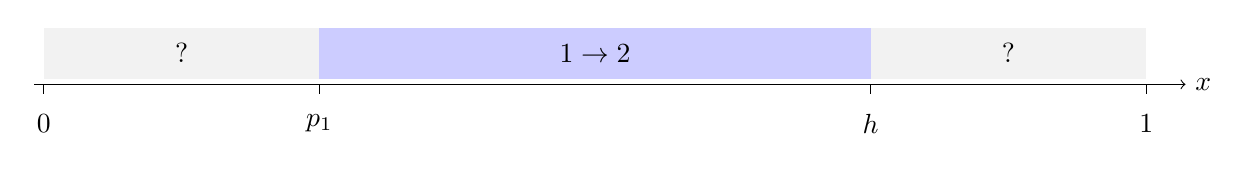
\begin{tikzpicture}[x=1cm,y=1cm]
\fill[gray!10] (0,0.07) rectangle (3.5,0.72);
\fill[blue!20] (3.5,0.07) rectangle (10.5,0.72);
\fill[gray!10] (10.5,0.07) rectangle (14,0.72);
\node at (1.75,0.395) {$?$};
\node at (7,0.395) {$1\to2$};
\node at (12.25,0.395) {$?$};
\draw[->] (-0.12,0) -- (14.5,0) node[right] {$x$};
\foreach \x/\lab in {0/0,3.5/p_1,10.5/h,14/1} {
  \draw (\x,0) -- (\x,-0.12);
  \node[below=4pt] at (\x,-0.12) {$\lab$};
}
\end{tikzpicture}
\label{fig:middle-interval-policy}
\end{figure}

\medskip\noindent\underline{\textbf{\boldmath Case $m\le p_1$.}}
In this case we study the regions $x\ge m$ and $x<m$ separately.

% \begin{figure}[H]
% \centering
% \begin{minipage}{0.48\textwidth}
% \centering
% \textbf{(a) $x\ge m$}\par\smallskip
% \begin{tikzpicture}[x=1cm,y=1cm]
% \fill[blue!20] (1,-0.13) rectangle (5,0.13);
% \draw[->] (-0.35,0) -- (5.45,0) node[right] {$x$};
% \foreach \x/\lab in {0/0,1/m,2.2/p_1,3.8/p_2,5/1} {
%   \draw (\x,-0.08) -- (\x,0.08);
%   \node[above=4pt] at (\x,0.08) {$\lab$};
% }
% \fill (1,0) circle (1.8pt);
% \end{tikzpicture}
% \end{minipage}\hfill
% \begin{minipage}{0.48\textwidth}
% \centering
% \textbf{(b) $x<m$}\par\smallskip
% \begin{tikzpicture}[x=1cm,y=1cm]
% \fill[blue!20] (0,-0.13) rectangle (1,0.13);
% \draw[->] (-0.35,0) -- (5.45,0) node[right] {$x$};
% \foreach \x/\lab in {0/0,1/m,2.2/p_1,3.8/p_2,5/1} {
%   \draw (\x,-0.08) -- (\x,0.08);
%   \node[above=4pt] at (\x,0.08) {$\lab$};
% }
% \draw[fill=white] (1,0) circle (1.8pt);
% \end{tikzpicture}
% \end{minipage}
% \end{figure}

For any $x\ge m$ every admissible trajectory stays in $[m,1]$ given that $m\le p_1\le p_2$ and so neither product can move the state across $m$ from above. Since $F$ decreases on this interval, product 1 is optimal there by trajectory ordering.
For $x<m$, since $m\le p_1$, this entire region lies below $p_1$. On $(0,a)$, where $F'<0$, Table $(*)$ permits only a $1\to2$ crossing, which implies that there can only exist one such crossing, given that after switching to product 2, returning to product 1 would require a $2\to1$ crossing, which is not possible on this interval. On $(a,m)$, where $F'>0$, the only permitted crossing is $2\to1$, so again there can be at most one.

Consequently, the only possible nonconstant pattern below $m$ is $1\to2\to1$ with either crossing possibly absent. Since product 1 is optimal from $m$ onward, product 2 is therefore optimal on at most one interval. The same argument applies when $m=p_1$, where product 1 can hold the state at the peak.

In this case we have prooved the only crossings that can happen are represented as  follows:

\begin{figure}[H]
\centering
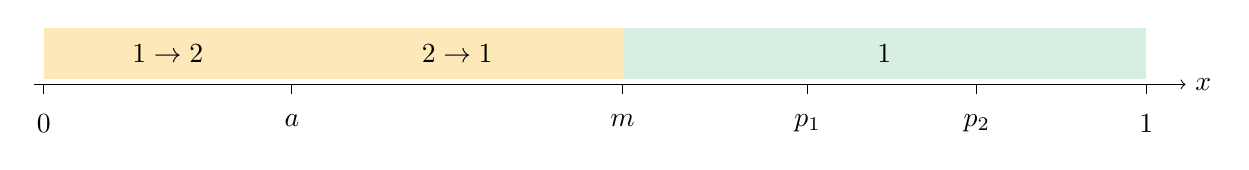
\begin{tikzpicture}[x=1cm,y=1cm]
\definecolor{policyStart}{HTML}{FCE8B8}
\definecolor{policyEnd}{HTML}{FCE8B8}
\definecolor{policyHold}{HTML}{D7EEE2}
\fill[policyStart] (0,0.07) rectangle (3.15,0.72);
\fill[policyEnd] (3.15,0.07) rectangle (7.35,0.72);
\fill[policyHold] (7.35,0.07) rectangle (14,0.72);
\node at (1.575,0.395) {$1\to2$};
\node at (5.25,0.395) {$2\to1$};
\node at (10.675,0.395) {$1$};
\draw[->] (-0.12,0) -- (14.5,0) node[right] {$x$};
\foreach \x/\lab in {0/0,3.15/a,7.35/m,9.7/p_1,11.85/p_2,14/1} {
  \draw (\x,0) -- (\x,-0.12);
  \node[below=4pt] at (\x,-0.12) {$\lab$};
}
\end{tikzpicture}
\end{figure}

\medskip\noindent\underline{\textbf{\boldmath Case $p_1<m\le p_2$.}}
Above $m$, product 1 is optimal. Fix $x>m$ and compare any admissible trajectory with the trajectory that uses product 1 until reaching $m$.
Since $b_1(x)<b_2(x)$ at every state, the product-1 trajectory is the smallest admissible trajectory and therefore reaches $m$ no later than the comparison trajectory. While both trajectories remain above $m$,
$F$ is decreasing, so the product-1 trajectory yields a weakly higher flow payoff.

If the product-1 trajectory reaches $m$ first, it can hold the state at $m$ until the comparison trajectory arrives. During this time it earns $F(m)$, which is at least the flow payoff of any state above $m$. Once both trajectories reach $m$, it can follow the same continuation. If the comparison trajectory never reaches $m$, holding at $m$ forever
is likewise weakly better. Hence any policy starting from $x>m$ is weakly dominated by one that uses product 1 until reaching $m$ and then continues optimally. Therefore, product 1 is optimal for every $x>m$.

On $[p_1,m]$, the preceding destination comparison gives at most one $1\to2$ crossing. We have proved then:

\begin{figure}[H]
\centering
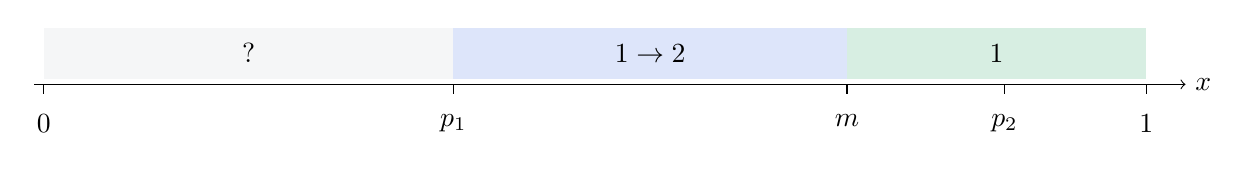
\begin{tikzpicture}[x=1cm,y=1cm]
\definecolor{policyUnknown}{HTML}{F5F6F7}
\definecolor{policyComparison}{HTML}{DDE5FA}
\definecolor{policyHold}{HTML}{D7EEE2}
\fill[policyUnknown] (0,0.07) rectangle (5.2,0.72);
\fill[policyComparison] (5.2,0.07) rectangle (10.2,0.72);
\fill[policyHold] (10.2,0.07) rectangle (14,0.72);
\node at (2.6,0.395) {$?$};
\node at (7.7,0.395) {$1\to2$};
\node at (12.1,0.395) {$1$};
\draw[->] (-0.12,0) -- (14.5,0) node[right] {$x$};
\foreach \x/\lab in {0/0,5.2/p_1,10.2/m,12.2/p_2,14/1} {
  \draw (\x,0) -- (\x,-0.12);
  \node[below=4pt] at (\x,-0.12) {$\lab$};
}
\end{tikzpicture}
\end{figure}

Now we prove that there cannot be a detached product-2 interval below $p_1$. Suppose first that $a>p_1$. Then $F'<0$ below $p_1$, so table $(*)$
allows only $1\to2$ crossings in this region. At $p_1$, if the low branch wins we have
\begin{equation*}
    W(p_1)=L(p_1)=\frac{F(p_1)}{\delta},
\end{equation*}
So 
\begin{equation*}
    g(p_1)= \delta W(p_1) - F(p_1) =0
\end{equation*}
If product 2 were optimal immediately to the left of $p_1$ we would have $b_2W'>b_1W'$. Since $0<b_1<b_2$ in this region, that would imply $W'>0$. Hence
\begin{equation*}
    g=b_2W'>0.
\end{equation*}
On this branch,
\begin{equation*}
    g'=\frac{\delta g}{b_2}-F'>0,
\end{equation*}
because $g>0$, $b_2>0$, and $F'<0$ in this region. Hence $g'>0$, so $g$ is strictly increasing as $x$ approaches $p_1$ from the left. This is incompatible with $g>0$ immediately to the left of $p_1$ and
$g(p_1)=0$. Therefore, product 2 cannot be optimal immediately to the left of $p_1$, and product 1 must be optimal there.

Since $a>p_1$, we have $F'<0$ throughout $(0,p_1)$, so Table $(*)$ allows only $1\to2$ crossings in this region. We have just shown that product 1 is optimal immediately to the left of $p_1$. Therefore, product 2 cannot be optimal at any lower state, otherwise, the policy would have to switch from product 2 back to product 1 before reaching $p_1$, requiring a $2\to1$ crossing, which is impossible.

\begin{figure}[H]
\centering
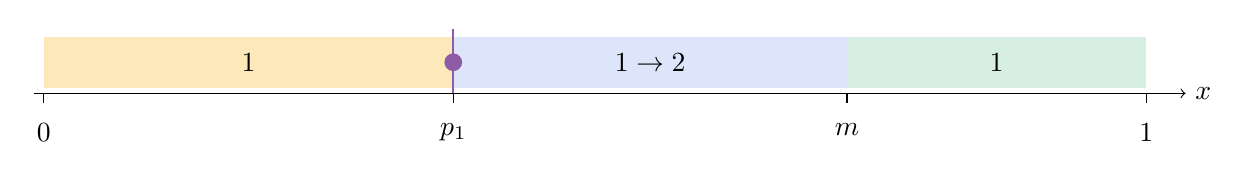
\begin{tikzpicture}[x=1cm,y=1cm]
\definecolor{policyLow}{HTML}{FCE8B8}
\definecolor{policyComparison}{HTML}{DDE5FA}
\definecolor{policyHold}{HTML}{D7EEE2}
\definecolor{policyBoundary}{HTML}{8E5BA6}
\fill[policyLow] (0,0.07) rectangle (5.2,0.72);
\fill[policyComparison] (5.2,0.07) rectangle (10.2,0.72);
\fill[policyHold] (10.2,0.07) rectangle (14,0.72);
\draw[policyBoundary,line width=0.8pt] (5.2,0) -- (5.2,0.82);
\fill[policyBoundary] (5.2,0.395) circle (3.2pt);
\node at (2.6,0.395) {$1$};
\node at (7.7,0.395) {$1\to2$};
\node at (12.1,0.395) {$1$};
\draw[->] (-0.12,0) -- (14.5,0) node[right] {$x$};
\foreach \x/\lab in {0/0,5.2/p_1,10.2/m,14/1} {
  \draw (\x,0) -- (\x,-0.12);
  \node[below=4pt] at (\x,-0.12) {$\lab$};
}
\end{tikzpicture}
\end{figure}

If instead the high branch strictly wins at $p_1$, then
\begin{equation*}
    W(p_1)=H(p_1)>L(p_1)=\frac{F(p_1)}{\delta},
\end{equation*}
so $g(p_1)= \delta W(p_1)-F(p_1)>0$. By continuity, $g>0$ immediately to the left of $p_1$ and since $0<b_1(x)<b_2(x)$ we have that 
\begin{equation*}
    g(x)=\max\{b_1(x)W'(x),\,b_2(x)W'(x)\}>0 \quad \Rightarrow \quad W'(x)>0
\end{equation*}
Therefore,
\begin{equation*}
    b_2(x)W'(x)>b_1(x)W'(x),
\end{equation*}
so product 2 is strictly optimal immediately to the left of $p_1$.

Because $a>p_1$, Table $(*)$ allows only $1\to2$ crossings below $p_1$. Hence any product-2 region on the left can begin at most once and must continue up to $p_1$. Since the high branch also uses product 2 immediately to the right of $p_1$, the two regions are connected and therefore form a single product-2 interval. Endpoint ties are treated separately below.

\begin{figure}[H]
\centering
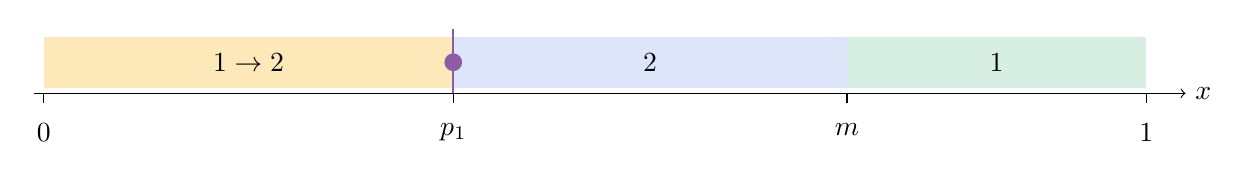
\begin{tikzpicture}[x=1cm,y=1cm]
\definecolor{policyLow}{HTML}{FCE8B8}
\definecolor{policyComparison}{HTML}{DDE5FA}
\definecolor{policyHold}{HTML}{D7EEE2}
\definecolor{policyBoundary}{HTML}{8E5BA6}
\fill[policyLow] (0,0.07) rectangle (5.2,0.72);
\fill[policyComparison] (5.2,0.07) rectangle (10.2,0.72);
\fill[policyHold] (10.2,0.07) rectangle (14,0.72);
\draw[policyBoundary,line width=0.8pt] (5.2,0) -- (5.2,0.82);
\fill[policyBoundary] (5.2,0.395) circle (3.2pt);
\node at (2.6,0.395) {$1\to2$};
\node at (7.7,0.395) {$2$};
\node at (12.1,0.395) {$1$};
\draw[->] (-0.12,0) -- (14.5,0) node[right] {$x$};
\foreach \x/\lab in {0/0,5.2/p_1,10.2/m,14/1} {
  \draw (\x,0) -- (\x,-0.12);
  \node[below=4pt] at (\x,-0.12) {$\lab$};
}
\end{tikzpicture}
\end{figure}

Now suppose that $a<p_1$. Since $p_1<m$, we have $F'>0$ throughout $(a,p_1)$. For any $x$ in this interval, product 1 moves the state upward
toward $p_1$, because $b_1(x)>0$. Along this trajectory the state remains in $(a,p_1)$, where $F$ is strictly increasing. Hence the subsequent flow
payoffs are strictly larger than $F(x)$, so
\begin{equation*}
    L(x)>\frac{F(x)}{\delta}.
\end{equation*}
Since by definition we have that $W(x)\geq L(x)$, it implies 
\begin{equation*}
    g(x)=\delta W(x)-F(x)>0.
\end{equation*}

Moreover, below $p_1$ we have $0<b_1(x)<b_2(x)$, so we have 
\begin{equation*}
    g(x)=\max\{b_1(x)W'(x),\,b_2(x)W'(x)\}>0 \quad \Rightarrow \quad W'(x)>0
\end{equation*}
Therefore,
\begin{equation*}
    b_2(x)W'(x)>b_1(x)W'(x),
\end{equation*}
So product 2 is strictly optimal throughout $(a,p_1)$.

Finally, on $(0,a)$ we have $F'<0$, so Table $(*)$ allows only $1\to2$ crossings. Since product 2 is already optimal immediately to the right of
$a$, any product-2 region below $a$ must connect to the one on $(a,p_1)$ and it cannot form a separate interval.

\begin{figure}[H]
\centering
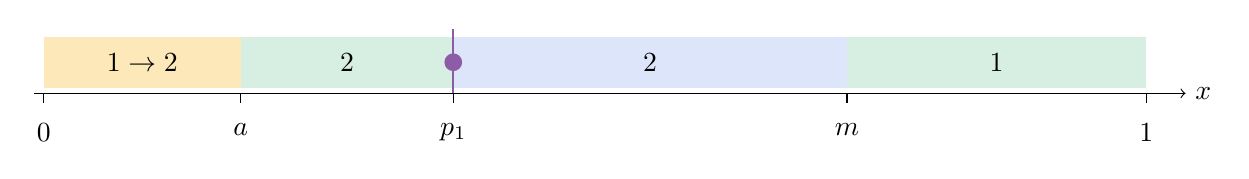
\begin{tikzpicture}[x=1cm,y=1cm]
\definecolor{policyLow}{HTML}{FCE8B8}
\definecolor{policyComparison}{HTML}{DDE5FA}
\definecolor{policyHold}{HTML}{D7EEE2}
\definecolor{policyBoundary}{HTML}{8E5BA6}
\fill[policyLow] (0,0.07) rectangle (2.5,0.72);
\fill[policyHold] (2.5,0.07) rectangle (5.2,0.72);
\fill[policyComparison] (5.2,0.07) rectangle (10.2,0.72);
\fill[policyHold] (10.2,0.07) rectangle (14,0.72);
\draw[policyBoundary,line width=0.8pt] (5.2,0) -- (5.2,0.82);
\fill[policyBoundary] (5.2,0.395) circle (3.2pt);
\node at (1.25,0.395) {$1\to2$};
\node at (3.85,0.395) {$2$};
\node at (7.7,0.395) {$2$};
\node at (12.1,0.395) {$1$};
\draw[->] (-0.12,0) -- (14.5,0) node[right] {$x$};
\foreach \x/\lab in {0/0,2.5/a,5.2/p_1,10.2/m,14/1} {
  \draw (\x,0) -- (\x,-0.12);
  \node[below=4pt] at (\x,-0.12) {$\lab$};
}
\end{tikzpicture}
\end{figure}

Finally, suppose that $a=p_1$, so that $p_1$ is the valley of $F$. Holding at $p_1$ yields the value $F(p_1)/\delta$, whereas moving toward the higher destination yields strictly larger subsequent values of $F$. Hence the high branch strictly wins at $p_1$, so $g(p_1)>0$. By continuity, product 2 is also optimal immediately to the left of $p_1$. Since $F'<0$ below $p_1$, Table $(*)$ allows only $1\to2$
crossings there, and any product-2 region on the left must therefore attach to the one at $p_1$. Hence product 2 can form at most one interval
below and across $p_1$.

The conclusion of this part can be illustrated it as follows: 

\begin{figure}[H]
\centering
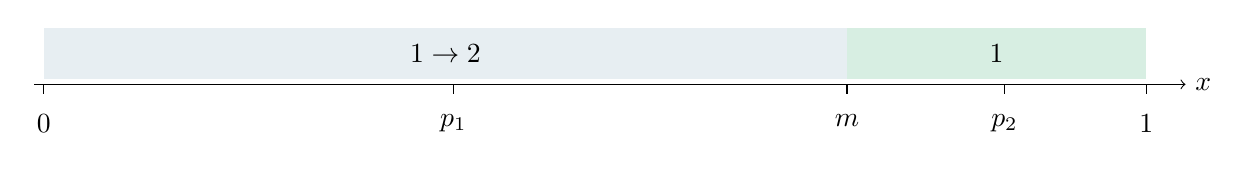
\begin{tikzpicture}[x=1cm,y=1cm]
\definecolor{policyJoined}{HTML}{E7EEF2}
\definecolor{policyHold}{HTML}{D7EEE2}
\fill[policyJoined] (0,0.07) rectangle (10.2,0.72);
\fill[policyHold] (10.2,0.07) rectangle (14,0.72);
\node at (5.1,0.395) {$1\to2$};
\node at (12.1,0.395) {$1$};
\draw[->] (-0.12,0) -- (14.5,0) node[right] {$x$};
\foreach \x/\lab in {0/0,5.2/p_1,10.2/m,12.2/p_2,14/1} {
  \draw (\x,0) -- (\x,-0.12);
  \node[below=4pt] at (\x,-0.12) {$\lab$};
}
\end{tikzpicture}
\end{figure}

\medskip\noindent\underline{\textbf{\boldmath Case $m>p_2$.}}
On $[p_1,p_2]$, the destination comparison applies with $h=p_2$, and the
preceding argument below $p_1$ is unchanged.

Suppose first that $a\geq p_2$. Any trajectory starting at $x\leq a$ remains below $a$, where $F$ is decreasing. Since product 1 generates the
smallest admissible trajectory, it is optimal throughout this region. For $x>a$, table $(*)$ allows only $1\to2$ crossings on $(a,m)$ and only
$2\to1$ crossings on $(m,1)$. Hence product 2 can be optimal on at most one interval. This case is illustrated as follows:


\begin{figure}[H]
\centering
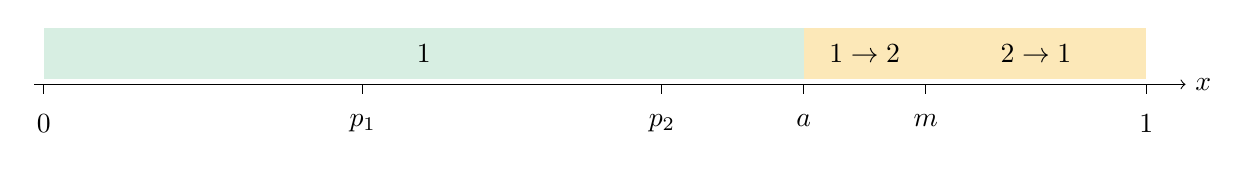
\begin{tikzpicture}[x=1cm,y=1cm]
\definecolor{policyHold}{HTML}{D7EEE2}
\definecolor{policyLow}{HTML}{FCE8B8}
\fill[policyHold] (0,0.07) rectangle (9.65,0.72);
\fill[policyLow] (9.65,0.07) rectangle (11.2,0.72);
\fill[policyLow] (11.2,0.07) rectangle (14,0.72);
\node at (4.825,0.395) {$1$};
\node at (10.425,0.395) {$1\to2$};
\node at (12.6,0.395) {$2\to1$};
\draw[->] (-0.12,0) -- (14.5,0) node[right] {$x$};
\foreach \x/\lab in {0/0,4.05/p_1,7.85/p_2,9.65/a,11.2/m,14/1} {
  \draw (\x,0) -- (\x,-0.12);
  \node[below=4pt] at (\x,-0.12) {$\lab$};
}
\end{tikzpicture}
\end{figure}


Now suppose that $a<p_2$. Then $F'>0$ on $(p_2,m)$, so table $(*)$ allows
only $1\to2$ crossings there. If the high destination strictly wins at
$p_2$, then
\begin{equation*}
    W(p_2)=H(p_2)=\frac{F(p_2)}{\delta},
\end{equation*}
and hence $g(p_2)=0$. Product 1 immediately to the right would require
$g>0$. On that branch, however,
\begin{equation*}
    g'=\frac{\delta g}{b_1}-F'<0,
\end{equation*}
since $b_1<0$ and $F'>0$. Thus a positive $g$ cannot emerge from $g(p_2)=0$, so product 2 remains optimal immediately to the right of $p_2$. Since no $2\to1$ crossing is possible before $m$, this product-2
region cannot split before reaching $m$.


\begin{figure}[H]
\centering
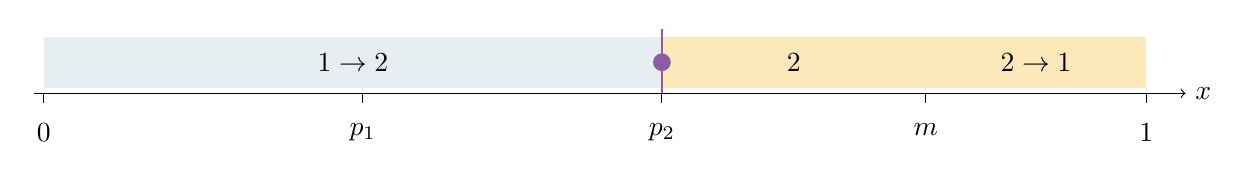
\begin{tikzpicture}[x=1cm,y=1cm]
\definecolor{policyJoined}{HTML}{E7EEF2}
\definecolor{policyLow}{HTML}{FCE8B8}
\definecolor{policyBoundary}{HTML}{8E5BA6}
\fill[policyJoined] (0,0.07) rectangle (7.85,0.72);
\fill[policyLow] (7.85,0.07) rectangle (11.2,0.72);
\fill[policyLow] (11.2,0.07) rectangle (14,0.72);
\draw[policyBoundary,line width=0.8pt] (7.85,0) -- (7.85,0.82);
\fill[policyBoundary] (7.85,0.395) circle (3.2pt);
\node at (3.925,0.395) {$1\to2$};
\node at (9.525,0.395) {$2$};
\node at (12.6,0.395) {$2\to1$};
\draw[->] (-0.12,0) -- (14.5,0) node[right] {$x$};
\foreach \x/\lab in {0/0,4.05/p_1,7.85/p_2,11.2/m,14/1} {
  \draw (\x,0) -- (\x,-0.12);
  \node[below=4pt] at (\x,-0.12) {$\lab$};
}
\end{tikzpicture}
\end{figure}

If instead the low destination strictly wins at $p_2$, then $L$ must win throughout $[p_1,p_2]$. Indeed, any interior crossing between $L$ and $H$ has orientation $L\to H$. Hence, if $H$ were to win at some state to the left of $p_2$, returning to $L$ before reaching $p_2$ would require an $H\to L$ crossing, which is impossible.

On $(p_2,m)$ we have $F'>0$, so Table $(*)$ allows only $1\to2$ crossings. Thus product 2 can begin at most once before $m$. For $x>m$, we have $F'<0$, so Table $(*)$ allows only $2\to1$ crossings, and the product-2 region can end at most once. Hence product 2 is optimal on at most one interval. Endpoint ties at $p_2$ are treated separately below.

\begin{figure}[H]
\centering
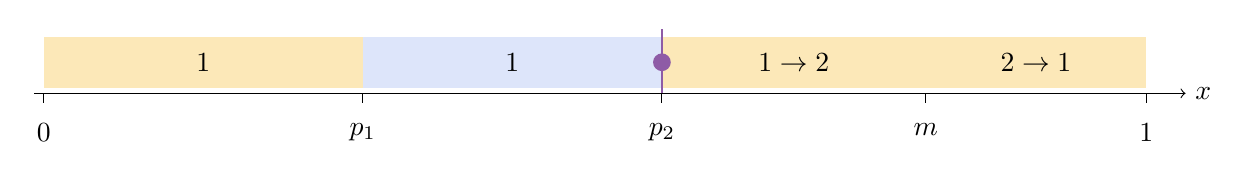
\begin{tikzpicture}[x=1cm,y=1cm]
\definecolor{policyLow}{HTML}{FCE8B8}
\definecolor{policyComparison}{HTML}{DDE5FA}
\definecolor{policyBoundary}{HTML}{8E5BA6}
\fill[policyLow] (0,0.07) rectangle (4.05,0.72);
\fill[policyComparison] (4.05,0.07) rectangle (7.85,0.72);
\fill[policyLow] (7.85,0.07) rectangle (11.2,0.72);
\fill[policyLow] (11.2,0.07) rectangle (14,0.72);
\draw[policyBoundary,line width=0.8pt] (7.85,0) -- (7.85,0.82);
\fill[policyBoundary] (7.85,0.395) circle (3.2pt);
\node at (2.025,0.395) {$1$};
\node at (5.95,0.395) {$1$};
\node at (9.525,0.395) {$1\to2$};
\node at (12.6,0.395) {$2\to1$};
\draw[->] (-0.12,0) -- (14.5,0) node[right] {$x$};
\foreach \x/\lab in {0/0,4.05/p_1,7.85/p_2,11.2/m,14/1} {
  \draw (\x,0) -- (\x,-0.12);
  \node[below=4pt] at (\x,-0.12) {$\lab$};
}
\end{tikzpicture}
\end{figure}

\medskip\noindent\textbf{Endpoint ties and threshold choices.}
It remains to consider ties between the two destinations that occur exactly at $p_1$ or $p_2$. These points require a separate argument because one of the drifts vanishes there. The cases in which $p_1$ or $p_2$ coincides with a valley or a peak of $F$ have already been covered: a valley at $p_1$ strictly favors the high destination, a valley at $p_2$ strictly favors the low destination, and peaks at either endpoint are included in the preceding cases.
Suppose first that
\begin{equation*}
    L(p_1)=H(p_1),\qquad h>p_1.
\end{equation*}
Recall that we have 
\begin{equation}
    L(p_1)=\frac{F(p_1)}{\delta} \quad \Rightarrow \quad H(p_1) = \frac{F(p_1)}{\delta}
    \label{eq:tie}
\end{equation}

Using the bellman equation of the high branch evaluated at $p_1$ gives
\begin{equation*}
    \delta H(p_1)=F(p_1)+b_2(p_1)H'(p_1) \quad \Rightarrow \quad b_2(p_1)H'(p_1) = 0 
\end{equation*}
And we obtain
\begin{equation*}
    b_2(p_1)=\lambda D(p_1)(p_2-p_1)>0 \quad \Rightarrow \quad H'(p_1)=0
\end{equation*}

For the low branch, the equation $\delta L=F+b_1L'$ does not directly determine $L'(p_1)$ because $b_1(p_1)=0$. We study then the derivative of the equation. Differentiating gives
\begin{equation*}
    \delta L' = F'+b_1'L'+b_1L''.
\end{equation*}
using that $b_1(p_1)=0$ and 
\begin{equation*}
    b_1'(p_1) = -\lambda D(p_1).
\end{equation*}
We obtain,
\begin{equation*}
    \bigl(\delta+\lambda D(p_1)\bigr)L'(p_1)= F'(p_1).
\end{equation*}
Note that a tie is only possible when $F'(p_1)<0$. Indeed, if $F'(p_1)>0$, moving to the right toward $h$ yields strictly larger subsequent values of $F$ than holding at $p_1$, so $H(p_1)>L(p_1)$. On the other hand, if $F'(p_1)=0$, since $h>p_1$, $p_1$ is the valley $a$, and the high destination again strictly improves on holding. Then, we must have $F'(p_1)<0$. Therefore,
\begin{equation*}
    L'(p_1)<0.
\end{equation*}
Hence
\begin{equation*}
    (H-L)'(p_1)>0,
\end{equation*}
so, starting from the tie at $p_1$, the high branch wins immediately to the right. Thus product 2 is optimal on that side.

It remains to determine the action immediately to the left. By eq \eqref{eq:tie} we have that $g(p_1)=0$. Suppose, by contradiction, that product 2 were optimal immediately to the
left of $p_1$. Since $0<b_1<b_2$ there, this would imply $W'>0$ and hence $g=b_2W'>0$. On this branch,
\begin{equation*}
    g'=\frac{\delta g}{b_2}-F'>0,
\end{equation*}
because $F'<0$. Thus $g$ would be strictly increasing as $x$ approaches $p_1$ from the left, which is incompatible with $g>0$ and $g(p_1)=0$. Therefore product 1 is optimal immediately to the left of $p_1$. The tie at $p_1$ consequently gives a $1\to2$ switch.

\begin{figure}[H]
\centering
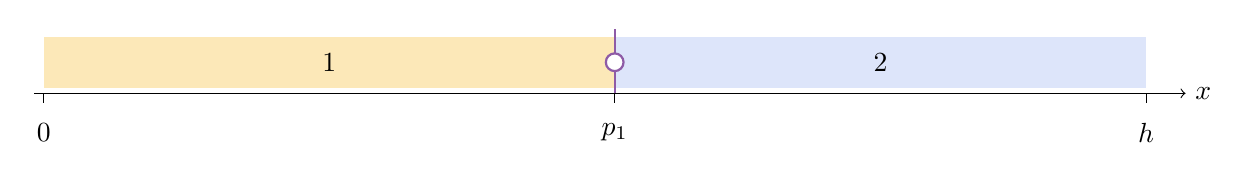
\begin{tikzpicture}[x=1cm,y=1cm]
\definecolor{policyLow}{HTML}{FCE8B8}
\definecolor{policyComparison}{HTML}{DDE5FA}
\definecolor{policyBoundary}{HTML}{8E5BA6}
\fill[policyLow] (0,0.07) rectangle (7.25,0.72);
\fill[policyComparison] (7.25,0.07) rectangle (14,0.72);
\draw[policyBoundary,line width=0.8pt] (7.25,0) -- (7.25,0.82);
\draw[policyBoundary,fill=white,line width=0.8pt] (7.25,0.395) circle (3.2pt);
\node at (3.625,0.395) {$1$};
\node at (10.625,0.395) {$2$};
\draw[->] (-0.12,0) -- (14.5,0) node[right] {$x$};
\foreach \x/\lab in {0/0,7.25/p_1,14/h} {
  \draw (\x,0) -- (\x,-0.12);
  \node[below=4pt] at (\x,-0.12) {$\lab$};
}
\end{tikzpicture}
\end{figure}

Now suppose that
\begin{equation*}
    L(p_2)=H(p_2),\qquad m>p_2.
\end{equation*}
Such a tie requires $F'(p_2)>0$. At the tie,
\begin{equation*}
    L'(p_2)=0,
    \qquad
    H'(p_2)>0,
\end{equation*}
so $(H-L)'(p_2)>0$. Since we approach $p_2$ from the left,
$H-L<0$ immediately before the tie, and therefore the low branch wins immediately to the left of $p_2$.

Again,
\begin{equation*}
    g(p_2)=0.
\end{equation*}
Suppose, by contradiction, that product 1 were optimal immediately to the right of $p_2$. Since $b_1<b_2<0$ there, this would imply $W'<0$ and hence $g=b_1W'>0$. On the product-1 branch,
\begin{equation*}
    g'=\frac{\delta g}{b_1}-F'<0,
\end{equation*}
because $b_1<0$ and $F'>0$. Hence a positive $g$ cannot emerge to the right from $g(p_2)=0$. Product 2 is therefore optimal immediately to the right of $p_2$, and the tie again gives a $1\to2$ switch.

\begin{figure}[H]
\centering
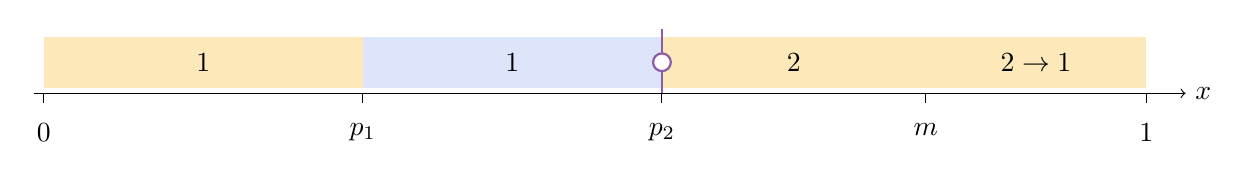
\begin{tikzpicture}[x=1cm,y=1cm]
\definecolor{policyLow}{HTML}{FCE8B8}
\definecolor{policyComparison}{HTML}{DDE5FA}
\definecolor{policyBoundary}{HTML}{8E5BA6}
\fill[policyLow] (0,0.07) rectangle (4.05,0.72);
\fill[policyComparison] (4.05,0.07) rectangle (7.85,0.72);
\fill[policyLow] (7.85,0.07) rectangle (11.2,0.72);
\fill[policyLow] (11.2,0.07) rectangle (14,0.72);
\draw[policyBoundary,line width=0.8pt] (7.85,0) -- (7.85,0.82);
\draw[policyBoundary,fill=white,line width=0.8pt] (7.85,0.395) circle (3.2pt);
\node at (2.025,0.395) {$1$};
\node at (5.95,0.395) {$1$};
\node at (9.525,0.395) {$2$};
\node at (12.6,0.395) {$2\to1$};
\draw[->] (-0.12,0) -- (14.5,0) node[right] {$x$};
\foreach \x/\lab in {0/0,4.05/p_1,7.85/p_2,11.2/m,14/1} {
  \draw (\x,0) -- (\x,-0.12);
  \node[below=4pt] at (\x,-0.12) {$\lab$};
}
\end{tikzpicture}
\end{figure}

At an interior tie between $L$ and $H$, either destination policy attains the same value, so either may be selected at the tie. If an attractive peak $m\in(p_1,p_2)$ is chosen as the destination, the state can be held at $m$ using the product-2 fraction
\begin{equation*}
    \frac{m-p_1}{p_2-p_1}.
\end{equation*}
With these choices at ties and holding thresholds, the optimal policy uses product 2 on at most one interval, completing the proof.
\end{proof}


An upper bound on the number of thresholds does not guarantee that any threshold exists. The following fixed-policy tests distinguish the two
constant-policy cases. Write $U^i_\rho$ for the fluid value obtained by always using product $i$:
\begin{equation*}
U^i_\rho(x)=(R-c_i)\int_0^\infty e^{-\delta t}D(x_i(t;x))\,dt.
\end{equation*}
% These functions are continuously differentiable. Indeed, fixed-policy trajectories converge uniformly exponentially to $p_i$, and their initial state derivatives are positive and eventually decay exponentially. One can therefore differentiate this integral under the integral sign. (explain this better)

\begin{corollary}[Existence of a nonconstant threshold policy]
\label{cor:fluid-nonconstant-threshold}
If we have 
\begin{align*}
\max_{x\in[0,1]}\{-\Delta c+\lambda\Delta p(U^1_\rho)'(x)\}&>0,\\
\min_{x\in[0,1]}\{-\Delta c+\lambda\Delta p(U^2_\rho)'(x)\}&<0.
\end{align*}
then there is an optimal policy with either one
or two interior thresholds, with one of the three patterns in
Theorem~\ref{lem:fluid-single-interval}.
\end{corollary}

\begin{proof}
For $i\in\{1,2\}$, the fixed-policy equation is
\begin{equation*}
\delta U^i_\rho(x)
=D(x)\left[R-c_i+\lambda(p_i-x)(U^i_\rho)'(x)\right].
\end{equation*}

\medskip\noindent\textbf{1. Rule out always using product 1.}
If this policy were optimal for every initial state, then $V=U^1_\rho$.
Subtracting its fixed-policy equation from \eqref{eq:fluid-HJB} gives
\begin{equation*}
0=D(x)\max\left\{0,-\Delta c+\lambda\Delta p(U^1_\rho)'(x)\right\}.
\end{equation*}
Since $D(x)>0$, this implies
\begin{equation*}
-\Delta c+\lambda\Delta p(U^1_\rho)'(x)\le0,
\qquad x\in[0,1].
\end{equation*}
Taking the maximum,
\begin{equation*}
\max_{x\in[0,1]}
\left\{-\Delta c+\lambda\Delta p(U^1_\rho)'(x)\right\}\le0,
\end{equation*}
contradicting the first hypothesis.

\medskip\noindent\textbf{2. Rule out always using product 2.}
If this policy were optimal for every initial state, then $V=U^2_\rho$.
The same subtraction now gives
\begin{equation*}
0=D(x)\max\left\{\Delta c-\lambda\Delta p(U^2_\rho)'(x),0\right\}.
\end{equation*}
Since $D(x)>0$,
\begin{align*}
\Delta c-\lambda\Delta p(U^2_\rho)'(x)&\le0,\\
-\Delta c+\lambda\Delta p(U^2_\rho)'(x)&\ge0,
\qquad x\in[0,1].
\end{align*}
Taking the minimum,
\begin{equation*}
\min_{x\in[0,1]}
\left\{-\Delta c+\lambda\Delta p(U^2_\rho)'(x)\right\}\ge0,
\end{equation*}
contradicting the second hypothesis.

\medskip\noindent\textbf{3. Apply the interval theorem.}
For the exact Beta demand, Lemma~\ref{lem:beta-marginal-demand}
and Proposition~\ref{lem:F-shape} establish the required payoff shape.
Theorem~\ref{lem:fluid-single-interval} therefore provides an optimal
interval policy. Since neither constant policy is optimal everywhere,
its pattern must be one of
\begin{equation*}
1\longrightarrow2,\qquad
2\longrightarrow1,\qquad
1\longrightarrow2\longrightarrow1.
\end{equation*}
These have, respectively, one, one, and two interior thresholds.
\end{proof}

\clearpage
\appendix
\section{Shape of the exact Beta demand}
\label{app:beta-demand}

\begin{lemma}[Shape of the exact Beta demand]\label{lem:beta-marginal-demand}
Let $0<p_0<1$, $0<\rho<1$, and $n=(1-\rho)^{-1}$. For
\begin{equation*}
D(x)=1-I_{p_0}\bigl(1+nx,1+n(1-x)\bigr),\qquad 0\le x\le1,
\end{equation*}
we have $D'(x)>0$ and
\begin{equation*}
D'(x)D'''(x)-[D''(x)]^2<0.
\end{equation*}
In particular, $D'$ is strictly log-concave. The endpoint derivatives are
understood through the smooth extension of $D$.
\end{lemma}

\begin{proof}
We establish a fixed-total Beta identity first. In this proof only, fix
$N>2$ and $p\in(0,1)$, write $b=N-a$, and let
\begin{equation*}
S(a)=1-I_p(a,b),\qquad 0<a<N.
\end{equation*}
For $0<h<b$, take a Dirichlet random vector $(U,Y,W)$ with parameters
$(a,h,b-h)$. Then $U$ has the Beta$(a,b)$ distribution, whereas $U+Y$
has the Beta$(a+h,b-h)$ distribution. Since $U+Y=1-W\ge U$,
\begin{equation*}
S(a+h)-S(a)=\Pr(U<p,\ W<1-p).
\end{equation*}
Integrating the Dirichlet density over this rectangle, dividing by $h$,
and letting $h\downarrow0$ gives
\begin{equation}\label{eq:beta-flux-positive}
S'(a)=\frac1{B(a,b)}
\int_0^p\int_0^{1-p}
\frac{u^{a-1}w^{b-1}}{1-u-w}\,dw\,du>0.
\end{equation}
Here $h\Gamma(h)\to1$. Dominated convergence is valid: the corner
singularity is proportional to
$\bigl[(p-u)+(1-p-w)\bigr]^{-1}$, which is integrable in two dimensions.
Choosing a fixed $h_0<b$ bounds the remaining integrand by a constant
times $u^{a-1}w^{b-h_0-1}/(1-u-w)$, also integrable.

Expand $(1-u-w)^{-1}$ into its nonnegative geometric series and use the
binomial theorem. Tonelli's theorem applied to
\eqref{eq:beta-flux-positive} yields
\begin{equation}\label{eq:beta-flux-series}
S'(a)=\sum_{j,k\ge0}t_{jk}(a),\qquad
 t_{jk}(a)=
\frac{p^a(1-p)^b}{B(a,b)}
\binom{j+k}{j}\frac{p^j(1-p)^k}{(a+j)(b+k)}.
\end{equation}
Let expectations and variances below use the probability weights
$t_{jk}(a)/S'(a)$. With $\psi$ and $\psi_1$ denoting the digamma and
trigamma functions, respectively, differentiation at fixed $a+b=N$
gives
\begin{equation*}
(\log t_{jk})'
=\log\frac p{1-p}-\psi(a)+\psi(b)
-\frac1{a+j}+\frac1{b+k},
\end{equation*}
and
\begin{equation*}
(\log t_{jk})''
=-\psi_1(a)-\psi_1(b)+\frac1{(a+j)^2}+\frac1{(b+k)^2}.
\end{equation*}
The logarithmic derivative of a positive sum therefore satisfies
\begin{align*}
(\log S')''
={}&-\psi_1(a)-\psi_1(b)
+\mathbb E\!\left[\frac1{(a+j)^2}+\frac1{(b+k)^2}\right]\\
&+\operatorname{Var}\!\left(-\frac1{a+j}+\frac1{b+k}\right).
\end{align*}
Termwise differentiation is justified on compact subintervals of
$(0,N)$: the summands and their first two derivatives are bounded by
a constant times the convergent positive summands at any fixed
interior parameter.

The variable in the variance lies in $[-1/a,1/b]$. Using the elementary
bound $\operatorname{Var}(Z)\le(M-m)^2/4$ when $Z\in[m,M]$, we obtain
\begin{equation}\label{eq:beta-logcurvature-bound}
(\log S')''
\le-\psi_1(a)-\psi_1(b)+\frac1{a^2}+\frac1{b^2}
+\frac14\left(\frac1a+\frac1b\right)^2.
\end{equation}
For every $s>0$, the trigamma series satisfies
\begin{equation*}
\psi_1(s)=\sum_{m=0}^{\infty}\frac1{(s+m)^2}
>\frac1s+\frac1{2s^2}.
\end{equation*}
Indeed, sum the strict trapezoidal inequality for the strictly convex
function $t\mapsto(s+t)^{-2}$ over $[m,m+1]$, $m\ge0$.

Suppose now that $a,b\ge1$. Put $A=1/a$ and $B=1/b$ for the following
algebra, so that $0<A,B\le1$. Equation
\eqref{eq:beta-logcurvature-bound} gives
\begin{align*}
(\log S')''
&<-(A+B)+\frac34(A^2+B^2)+\frac12AB\\
&\le-\frac14(A^2+B^2)+\frac12AB
=-\frac14(A-B)^2\le0,
\end{align*}
where the second inequality uses $A+B\ge A^2+B^2$.
The first inequality is strict, including when $A=B$.

Finally, take $N=n+2$, $p=p_0$, and $a=1+nx$. Both $a$ and
$b=1+n(1-x)$ are at least one on $[0,1]$. Since
$D'(x)=nS'(1+nx)$, positivity and strict log-concavity follow from
the preceding calculation.
\end{proof}

\end{document}
